% Compile: pdflatex main.tex twice. Requires elsarticle and ./figures/*.png.
\documentclass[preprint,3p,times]{elsarticle}
% elsarticle's legacy Times setup needs an explicit Unicode-engine font.
\usepackage{iftex}
\ifPDFTeX
  \usepackage[T1]{fontenc}
  \usepackage[utf8]{inputenc}
\else
  \usepackage{fontspec}
  \setmainfont{texgyretermes}[Extension=.otf,
    UprightFont=*-regular,BoldFont=*-bold,
    ItalicFont=*-italic,BoldItalicFont=*-bolditalic]
  \setmonofont{lmmono10-regular.otf}
\fi
\usepackage{amsmath,amssymb}
\usepackage{graphicx}
\usepackage{booktabs,multirow}
\usepackage{enumitem}
\usepackage{xurl}
\usepackage{placeins}
\usepackage[hidelinks,breaklinks]{hyperref}
\hypersetup{pdfauthor={Oussama Hichou; Abdelhak Tali; Abderrahim El Inaji},
  pdftitle={One-class ECG verification using wavelet features and a compact Kolmogorov--Arnold autoencoder}}
\urlstyle{same}
\setlength{\emergencystretch}{1em}
\renewcommand{\topfraction}{0.9}
\renewcommand{\bottomfraction}{0.8}
\renewcommand{\textfraction}{0.08}
\renewcommand{\floatpagefraction}{0.65}
% Avoid the extra trailing space in older elsarticle title-page footers.
\makeatletter
\def\ps@pprintTitle{%
  \let\@oddhead\@empty\let\@evenhead\@empty
  \def\@oddfoot{\footnotesize\itshape
    Preprint submitted to \@journal\hfill\@date}%
  \let\@evenfoot\@oddfoot}
\makeatother
\graphicspath{{./figures/}{../paper/figures/}}
\journal{Biomedical Signal Processing and Control}
\begin{document}
\begin{frontmatter}
\title{One-class ECG verification using wavelet features
and a compact Kolmogorov--Arnold autoencoder}
\author[a]{Oussama Hichou\corref{cor1}}
\ead{oussama.hichou@etu.uae.ac.ma}
\cortext[cor1]{Corresponding author.}
\author[a]{Abdelhak Tali}
\ead{atali@uae.ac.ma}
\author[a]{Abderrahim El Inaji}
\ead{a.elinaji@uae.ac.ma}
\affiliation[a]{organization={Lab TIC, Universit\'e Abdelmalek Essa\^adi},
city={Tangier},country={Morocco}}
\begin{abstract}
Electrocardiogram (ECG) verification decides whether a heartbeat comes from
the person who claims an identity. When enrolment relies on one short
recording, the verifier has to be learned from a few dozen genuine beats and
without impostor examples. We study this one-class setting on ECG-ID. Each
beat is summarised by 26 values derived from the maxima ridges
of its continuous wavelet transform, and this summary is compared with a
PCA-reduced waveform input across four classical novelty detectors and two
autoencoders: a multilayer perceptron (MLP) and a compact Kolmogorov--Arnold
network (KAN) with learned spline connections. In an exploratory within-recording
test on 30 participants, the wavelet summary raised the mean area
under the ROC curve (AUROC) for five of the six models. The KAN autoencoder
reached a mean AUROC of 0.977 and an equal error rate (EER) of 0.054 with
3{,}248 trainable parameters, compared with 8{,}422 for the MLP. Its ranking
performance was very close to that of the MLP, which gave the same AUROC for
27 of the 30 participants, and to that of a one-class support vector machine;
the paired 95\% intervals for both AUROC differences lay within $\pm0.006$.
With a threshold set from enrolment beats alone, the KAN had the highest mean
$F_1$ score (0.875), although its advantage over the MLP was not clear. On
separate same-day recordings from ten participants, the KAN reached an AUROC
of 0.952 and an EER of 0.086 with Morlet-based features. These results still
need confirmation on unseen participants and later recording sessions.
\end{abstract}
\begin{keyword}
ECG biometrics \sep wavelet transform modulus maxima \sep continuous wavelet
transform \sep one-class classification \sep Kolmogorov--Arnold networks
\sep anomaly detection
\end{keyword}
\end{frontmatter}

\section{Introduction}\label{sec:intro}
The electrocardiogram (ECG) reflects the electrical activity of the heart.
Because beat morphology differs from one person to another, the ECG has been
proposed as a biometric trait \cite{melzi2022}. It has to be measured from
the body, but this does not make it immune to attack: stored or synthesised
signals can be replayed to a verification system \cite{karimian2020}.

A practical difficulty arises at enrolment. A new user may supply only one
short recording, and the system must learn from it what that user's beats
look like. No examples from impostors are available at this stage, so the
problem is one of \emph{one-class learning}: the model sees genuine data only
and must later judge whether an unfamiliar beat fits. One-class support
vector machines (OC-SVMs) have been applied to ECG verification in this way
\cite{hejazi2017,galli2020}.

How each beat is represented largely determines what such a model can learn.
The P wave, QRS complex and T wave occupy different time intervals and
frequency ranges \cite{clifford2006}, and the continuous wavelet transform
(CWT) describes both at once. Local maxima of the CWT modulus can be followed
from coarse to fine scales, forming \emph{maxima ridges} that mark sharp
signal changes \cite{mallat1992,mallat1999}. Ridge analysis has already been
used to characterise ECG beats and to measure intervals between them
\cite{legarreta2005}.

In this work, every beat is reduced to 26 numbers that summarise its maxima
ridges in five frequency bands. We compare this summary with a PCA-reduced
waveform across six one-class models. Four are classical novelty detectors;
the other two are autoencoders, that is, networks trained to reproduce their
own input \cite{ruff2021}. An autoencoder fitted to one person's beats tends
to reproduce new beats from the same person well, so a large reconstruction
error is evidence that a beat belongs to someone else.

Our main interest is an autoencoder built from a Kolmogorov--Arnold network
(KAN) \cite{liu2024}. Instead of a fixed activation after each weighted sum,
a KAN places a small learned function on every connection. With so few
enrolment beats, the question is whether such a network can match a
conventional MLP autoencoder while using fewer trainable parameters. We make
no assumption either way, because published KAN--MLP comparisons depend
strongly on the task and on how model size is controlled \cite{yu2024}.

The contributions of the study are:
\begin{enumerate}[label=(\roman*)]
\item a 26-value wavelet-ridge summary for learning an ECG verifier from one
      person's beats;
\item a comparison of six one-class models on 30 ECG-ID participants, with
      per-participant results and bootstrap uncertainty intervals;
\item a paired comparison of a compact KAN autoencoder with an MLP
      autoencoder that has 2.6 times as many parameters;
\item a test on a second recording for ten participants, using two wavelets.
\end{enumerate}
Model ranking is assessed mainly with AUROC and EER. We also report $F_1$ at
a threshold derived from enrolment beats only, which mimics a deployed
system. Because some participants contributed to the choice of model settings
(Section~\ref{sec:development}), all results should be read as exploratory.

\section{Related work}\label{sec:related}
\subsection{ECG identity recognition}
Early work by Israel et~al.\ \cite{israel2005} identified individuals from
measured ECG intervals and amplitudes. Later studies turned wavelet
coefficients into images: Byeon et~al.\ \cite{byeon2019} trained deep models
on scalograms. El Boujnouni et~al.\ applied capsule networks first to
scalograms \cite{elboujnouni2020} and later to wavelet features extracted from
the PTB, MIT-BIH Arrhythmia, MIT-BIH Normal Sinus Rhythm and MIT-BIH ST Change
databases \cite{elboujnouni2022}. These are identification studies, in which
the classifier is trained on every enrolled person.

Wavelet representations are also common in clinical ECG classification; for
instance, Ozaltin and Yeniay \cite{ozaltin2023} classified scalograms of
arrhythmia, heart-failure and normal-rhythm recordings with a CNN--SVM model.
That task concerns diagnosis rather than identity. Melzi et~al.\
\cite{melzi2022} review ECG biometrics and show how strongly reported
performance depends on recording conditions and evaluation design.

Verification from genuine data alone has been addressed before. Hejazi
et~al.\ \cite{hejazi2017} applied an OC-SVM to non-fiducial ECG features, and
Galli et~al.\ \cite{galli2020} combined Gaussian-model ECG features with an
optimised OC-SVM. Bhuva and Kumar \cite{bhuva2023} considered continuous
authentication for Internet-of-Things devices. The present study stays within
this one-class framework and examines a specific ridge summary and a KAN
autoencoder.

\subsection{Wavelet maxima}
Mallat and Hwang \cite{mallat1992} showed that the maxima of the wavelet
transform modulus locate singularities and sharp transitions, and that
following them across scales characterises the local regularity of a signal
\cite{mallat1999}. Legarreta et~al.\ \cite{legarreta2005} brought this
analysis to ECG beat characterisation and beat-to-beat measurement. We use
the ridges only as a source of summary statistics; no multifractal spectrum
is estimated.

\subsection{One-class detectors}
The classical detectors in our comparison judge similarity to the enrolment
data in different ways. An OC-SVM learns a boundary that encloses most of the
training data in a kernel space \cite{scholkopf2001}, an idea closely related
to support vector data description \cite{tax2004}. Isolation Forest scores a
sample by how quickly random axis-parallel splits isolate it \cite{liu2008}.
The local outlier factor (LOF) compares the density around a sample with that
around its neighbours \cite{breunig2000}. Elliptic Envelope fits a robust
Gaussian model and uses the Mahalanobis distance from its centre.
Autoencoders, in contrast, judge a sample by how well they can reconstruct it
\cite{ruff2021}. Contrastive approaches such as CLOCS \cite{kiyasseh2021}
learn cardiac representations from many patients and therefore follow a
different training paradigm.

\subsection{Kolmogorov--Arnold networks in cardiac signal analysis}
KANs replace fixed node activations with learnable univariate functions on
the network edges \cite{liu2024}. KAN autoencoders have been explored for
image reconstruction \cite{moradi2024}, and KAN-AD applies Fourier-based KAN
layers to time-series anomaly detection \cite{zhou2025kanad}. Closest to our
setting, Lomoio et~al.\ \cite{lomoio2025} compared KAN and conventional
autoencoders on heart-sound recordings, including anomaly detection, although
their input is stethoscope audio rather than ECG. Other cardiac applications,
such as KACQ-DCNN for heart-disease detection \cite{jahin2025} and MAK-Net for
arrhythmia classification \cite{zhao2025}, embed KAN layers in larger
supervised models trained on labelled clinical classes. None of these studies
indicates how a small KAN autoencoder behaves when it is fitted to the beats
of a single person. We therefore compare it directly with an MLP autoencoder
and with classical detectors, and we report model size explicitly
\cite{yu2024}.

\section{Data and evaluation protocol}\label{sec:data}
\subsection{The ECG-ID database}
ECG-ID \cite{lugovaya2005}, distributed through PhysioNet
\cite{goldberger2000,pollard2026}, contains 310 lead-I recordings from 90
volunteers. Each recording lasts about 20\,s and is sampled at 500\,Hz. Every
record holds an unfiltered and a filtered channel; we use the unfiltered
first channel and apply our own cleaning (Section~\ref{sec:cleaning}).

The main experiment uses the first recording (\texttt{rec\_1}) of
Persons~01--30. After beat extraction these recordings yield 747 complete
beats, between 17 and 39 per person. A 70/30 split leaves 11--27 enrolment
beats and 6--12 genuine test beats per person. Table~\ref{tab:dataset}
summarises both test protocols.
\begin{table}[htbp]
\centering
\caption{The ECG-ID data and the two test protocols.}\label{tab:dataset}
\begin{tabular}{ll}\toprule
Property & Value \\\midrule
Participants / recordings in ECG-ID & 90 / 310 \\
Sampling frequency / lead & 500\,Hz / I \\
Recording duration & Approximately 20\,s \\
Main experiment participants & \texttt{Person\_01}--\texttt{Person\_30} \\
Main recording & \texttt{rec\_1} \\
Usable beats & 17--39 per participant; 747 total \\
Within-recording split & 70\% enrolment; 30\% genuine probes \\
Impostor probes & Same count as genuine probes; other participants \\
Second-recording experiment & 10 development participants \\
Second-recording enrolment / probes & \texttt{rec\_1} / \texttt{rec\_2} \\\bottomrule
\end{tabular}
\end{table}

\subsection{Enrolment and test beats}\label{sec:development}
In the within-recording test, each person's beats are shuffled and the first
$\lfloor0.70n\rfloor$ of the $n$ beats form the enrolment set, with at least
three enrolment beats and one test beat guaranteed. The remaining beats serve
as genuine probes. An equal number of impostor probes is drawn from the
\texttt{rec\_1} beats of the other 29 participants, with replacement only if
that pool is too small. Person~$i$ (counting from $i=0$ for Person~01) uses
the seed $42+i$ for both this split and the later neural validation split.
All six models, and both input types, therefore see exactly the same
enrolment beats and probes for a given person. The global run seed (42 by
default) does not affect these per-person seeds or the fixed random states of
the classical detectors.

Everything that is learned from data, including the feature scaler, the
waveform PCA and the acceptance threshold, is fitted on enrolment beats only.
Test labels play no part in setting the threshold. Neural weights are trained
on an enrolment subset, and the remaining enrolment beats may be used for
early stopping; the KAN spline grids are fitted on the training subset alone.
One caveat concerns preprocessing: the signal is cleaned and segmented as a
whole before beats are divided, so enrolment and test beats are not separate
acquisitions.

Model settings were chosen once for all participants, and the separation
between development and evaluation data is incomplete. Persons~01--10 were
designated as the development group, yet the saved design comparison
(\texttt{results/kan\_design\_ablation.csv}) also contains Gaussian and Morlet
results for Persons~11--30. No dated log records which of these results, or
whether any second-recording result, were examined before the settings were
fixed. For this reason, we treat all three experiments as exploratory and do
not present Persons~11--30 as an untouched test group.
Table~\ref{tab:cohorts} reports the two groups separately for transparency.

\subsection{Acceptance threshold}\label{sec:threshold}
Each detector assigns a score to a new beat. For the classical detectors a
higher score indicates a closer match, and the threshold for person $u$ is the
lowest score observed on that person's enrolment set $\mathcal E_u$:
\begin{equation}
 t_u=\min_{x\in\mathcal E_u}s_u(x),\qquad
 \widehat y_u(x)=\mathbb I\{s_u(x)\ge t_u\}.
 \label{eq:threshold}
\end{equation}
Scores come from \texttt{score\_samples}, or from \texttt{decision\_function}
where the former is unavailable. For the autoencoders a lower reconstruction
error indicates a closer match, and the threshold is the largest error on the
enrolment set, including beats held out for early stopping. In both cases the
rule (the 100th percentile of enrolment scores) accepts every enrolment beat.
It is simple and needs no impostor data, but it need not be equally suitable
for every model. Because each person has as many impostor probes as genuine
ones, $F_1$ values are comparable across models in this study; they would
change under a different genuine-to-impostor ratio.

\subsection{Testing with a second recording}\label{sec:crossproto}
The second protocol uses Persons~01--10. All usable beats of \texttt{rec\_1}
serve for enrolment and all usable beats of \texttt{rec\_2} as genuine
probes, together with the same number of impostor beats drawn from the other
participants' \texttt{rec\_2}. Over the ten people this gives 239 enrolment
beats, 241 genuine probes and 241 impostor probes.

The ECG-ID headers list the same acquisition date for \texttt{rec\_1} and
\texttt{rec\_2} of all ten participants. This protocol therefore tests
separate recordings made on the same day. It does not test stability over days
or months, and the headers do not reveal the interval between recordings or
whether the electrodes were repositioned. As these participants also belong to
the development group, the test is not independent confirmation.

\subsection{Performance measures}
We report three measures:
\begin{itemize}
\item \textbf{AUROC} is the probability that a randomly chosen genuine probe
      receives a better score than a randomly chosen impostor probe. It does
      not depend on any threshold; 0.5 corresponds to chance and 1.0 to a
      perfect ranking of the test set.
\item \textbf{$F_1$} is the harmonic mean of precision (the share of accepted
      probes that are genuine) and recall (the share of genuine probes that
      are accepted), evaluated at the enrolment threshold of
      Eq.~\eqref{eq:threshold}.
\item \textbf{EER} is the error rate at which false acceptance and false
      rejection are equal. With so few probes the two rates rarely coincide
      exactly, so we take the ROC point where they are closest and report
      their mean, without interpolation.
\end{itemize}
The EER threshold is chosen on the test data and so describes the attainable
trade-off, whereas $F_1$ reflects the threshold a deployed system would
actually use.

All summaries average over participants, so each person carries the same
weight. Ninety-five per cent confidence intervals come from a participant
bootstrap: participants are resampled with replacement 10{,}000 times, the
mean is recomputed each time, and the 2.5th and 97.5th percentiles are
retained. Paired comparisons with the KAN resample per-person differences in
the same way. An interval that contains zero indicates that the data do not
resolve a difference; it does not show that two models are equivalent.
Per-person values are rounded to four decimals before summarising, no
correction for multiple comparisons is applied, and the bootstrap does not
capture uncertainty from model selection, training seeds or the shared
impostor pool.

\section{Method}\label{sec:method}
Figure~\ref{fig:stages} follows one beat through the processing chain:
detection in the recording, extraction of a fixed window, the wavelet power
map and the maxima ridges from which the 26 features are computed. A separate
verifier is then fitted for each enrolled person.
\begin{figure}[htbp]\centering
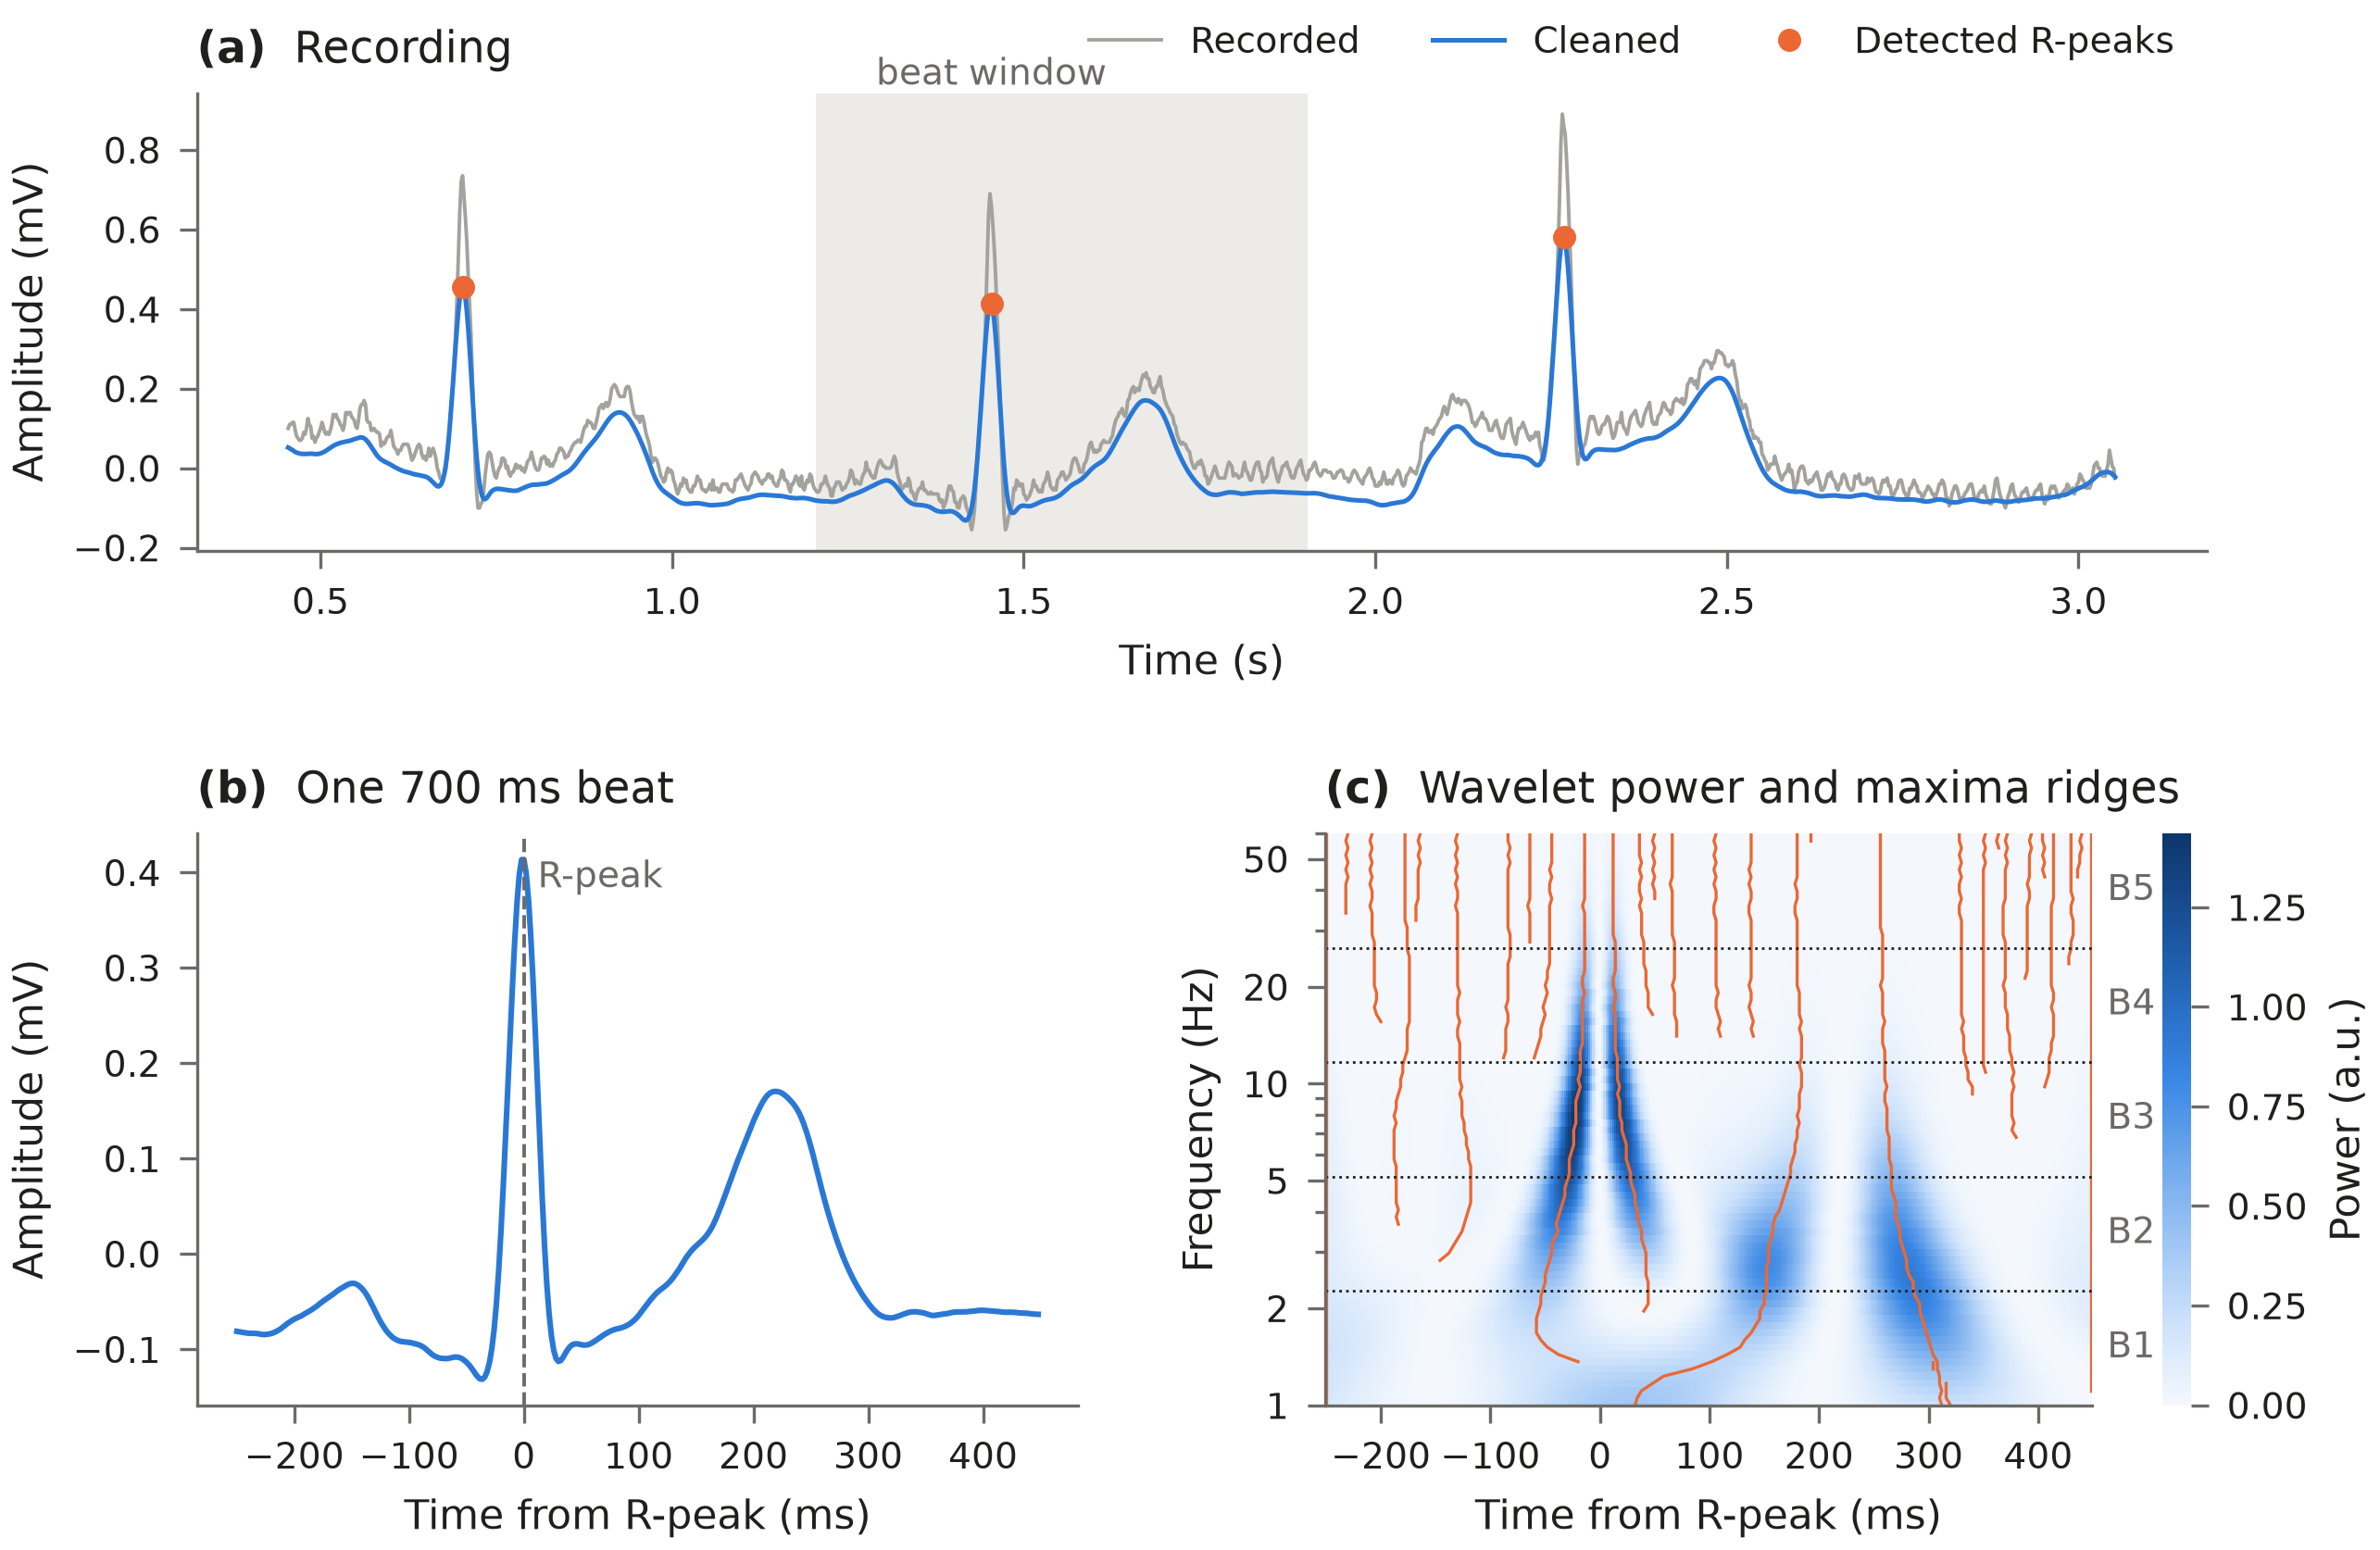
\includegraphics[width=\textwidth]{fig_stages.png}
\caption{Processing of one beat from Person~01. (a)~Recorded and cleaned
signal with detected R-peaks; the shaded band marks the 700\,ms beat window.
(b)~The extracted beat. (c)~Wavelet power of the beat (first Gaussian
derivative wavelet) with its maxima ridges in orange. Dotted lines separate
the five frequency bands B1--B5 used to summarise the ridges.}
\label{fig:stages}
\end{figure}

\subsection{Cleaning and beat extraction}\label{sec:cleaning}
Signals are processed with the default \texttt{neurokit} method of
\texttt{nk.ecg\_process} in NeuroKit2 \cite{makowski2021}, which supplies the
cleaned signal and the R-peak locations. According to the library
documentation, this method removes baseline drift with a 0.5\,Hz high-pass
Butterworth filter of order five and then suppresses 50\,Hz mains
interference. Its R-peak detector locates QRS complexes from the steepness of
the signal, unlike the Pan--Tompkins algorithm \cite{pan1985}, and the
processing call also applies the library's peak correction. Package versions
were not recorded for the original runs, so these details describe the
documented defaults rather than a verified historical installation. With the
current release (NeuroKit2~0.2.13), the beats and wavelet features of the
main experiment are reproduced to within a relative difference of
$10^{-7}$.

Around each R-peak, a window from 250\,ms before to 450\,ms after the peak is
cut with \texttt{nk.epochs\_create}, giving 350 samples at 500\,Hz. Windows
that extend past either end of the recording contain missing values and are
discarded.

The two inputs treat amplitude differently. For the waveform input, each beat
is standardised individually (mean removed, then divided by its standard
deviation plus $10^{-8}$). The wavelet input is computed from the cleaned beat
without this step, so it retains amplitude information. Both inputs are later
standardised with statistics from the enrolment beats. The comparison is thus
between two complete input pipelines and does not isolate the contribution of
the wavelet summary alone.
\begin{figure}[htbp]\centering
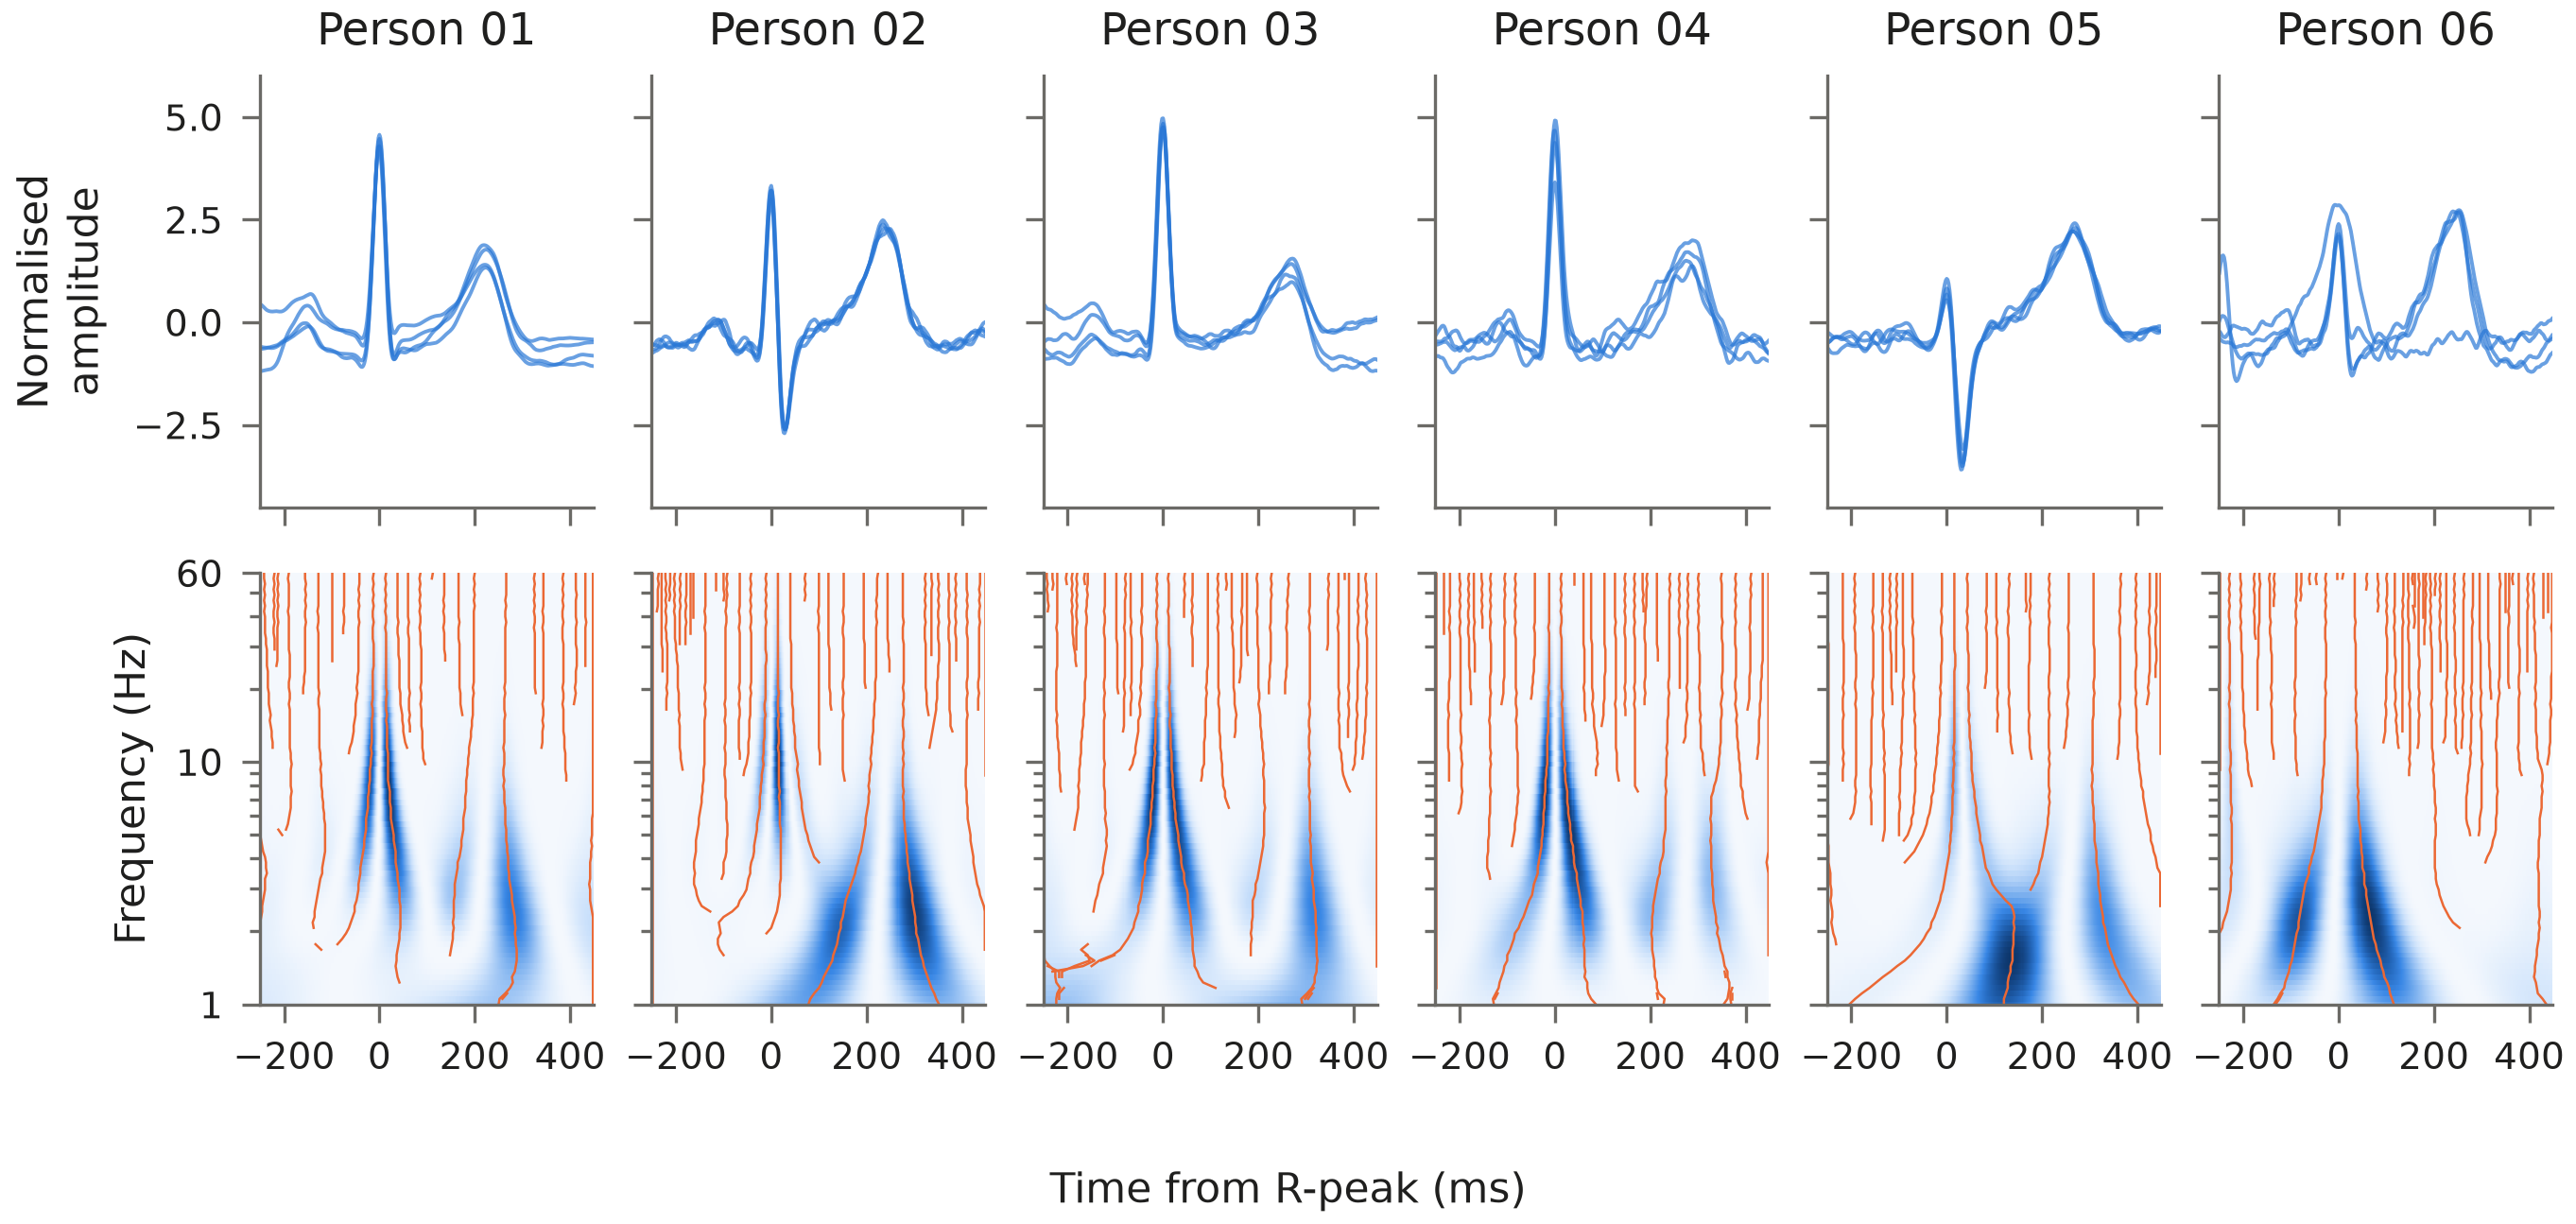
\includegraphics[width=\textwidth]{fig_beats.png}
\caption{Beats and wavelet ridges for Persons~01--06. Top: four individually
standardised beats per person, overlaid. Bottom: wavelet power of the first
(unstandardised) beat with its maxima ridges; colour scales are set per
panel. One of the four beats of Person~06 has an atypical shape.}
\label{fig:beats}
\end{figure}

\subsection{Wavelet power map}
The CWT of a beat $b(t)$ is
\begin{equation}
\mathcal W_b(a,\tau)=\frac{1}{\sqrt a}
 \int b(t)\,\psi^*\!\left(\frac{t-\tau}{a}\right)\mathrm dt,
 \label{eq:cwt}
\end{equation}
where $\psi$ is the mother wavelet, the scale $a$ stretches it and the shift
$\tau$ moves it along the beat; the factor $1/\sqrt a$ keeps the wavelet
energy constant across scales. We compute the transform with the
convolution-based \texttt{cwt} routine of PyWavelets at 80 frequencies spaced
logarithmically between 1 and 60\,Hz, converting each frequency $f$ to a scale
$a=f_c f_s/f$, where $f_c$ is the centre frequency of the wavelet and $f_s$
the sampling rate. The squared modulus $|\mathcal W_b|^2$ is referred to below
as wavelet power.

The main experiments use the first derivative of a Gaussian (\texttt{gaus1}),
the classical choice for modulus-maxima analysis \cite{mallat1992,mallat1999};
the second-recording test also uses the real Morlet wavelet (\texttt{morl}).
No padding or edge correction is applied. At the lowest frequencies the
wavelet is longer than the 700\,ms window, so these coefficients are strongly
influenced by the window edges.

\subsection{From maxima ridges to 26 features}
Within each frequency row of the power map, a time point is a local maximum if
its power exceeds that of both neighbours (or of its single neighbour at
either end). Maxima are then chained from the coarsest to the finest scale:
from its current position, a chain moves to the nearest unused maximum in the
next row, provided that it lies within $\max(1,\operatorname{round}(a/2))$
samples, and stops when no such maximum exists. Ties go to the earlier time
point. Maxima become unavailable once they are used, even if their chain is
later discarded for spanning fewer than two rows.

Let $L$ denote the number of retained ridges. The 1--60\,Hz range is divided
into five logarithmic bands with edges at approximately 1, 2.27, 5.14, 11.67,
26.46 and 60\,Hz (B1--B5 in Fig.~\ref{fig:stages}c). For each band $k$ we
record
\begin{enumerate}
\item the number $C_k$ of ridges with at least one point in the band;
\item the mean $\bar f_k$ and population standard deviation $\sigma_{f,k}$ of
      the frequencies of those ridge points;
\item the mean $\bar p_k$ and population standard deviation $\sigma_{p,k}$ of
      their wavelet power.
\end{enumerate}
Statistics are pooled over all in-band points, so long ridges carry more
weight than short ones. Band limits are inclusive, which lets a point that
falls exactly on an edge count in both bands, and an empty band contributes
zeros. Together with $L$, this gives the feature vector
\begin{equation}
\mathbf v(b)=\bigl[L,C_1,\bar f_1,\sigma_{f,1},\bar p_1,\sigma_{p,1},
\ldots,C_5,\bar f_5,\sigma_{f,5},\bar p_5,\sigma_{p,5}\bigr]
\in\mathbb R^{26}.\label{eq:features}
\end{equation}
The summary borrows the ridge construction of WTMM analysis but does not
estimate a multifractal spectrum.

For both inputs, \texttt{StandardScaler} centres and scales each feature with
the enrolment mean and standard deviation. The waveform input is then
projected by PCA, fitted on the enrolment beats, onto
$\min(40,n_{\rm enrol},350)$ components without whitening. Because PCA centres
the data, at most $n_{\rm enrol}-1$ of these components can have non-zero
variance; with 11--27 enrolment beats, the waveform input therefore carries
at most 26 informative dimensions, and possibly fewer.

\subsection{Classical detectors}
The four classical detectors are taken from scikit-learn with the settings in
Table~\ref{tab:settings}; all other options keep their library defaults. Their
built-in decision thresholds are not used. Instead, every model is thresholded
with the enrolment rule of Eq.~\eqref{eq:threshold}. When a person has fewer
enrolment beats than input features, the covariance estimate of Elliptic
Envelope can be unstable. The original script suppressed warnings and would
have dropped failed fits silently; however, the saved tables contain finite
results for all six models and both inputs, for 30 people in the main test
and ten in each second-recording test. The released code now keeps warnings,
records failures and stops if any result is missing.
\begin{table}[htbp]\centering
\caption{Model and training settings. $d$ is the input dimension after
enrolment-fitted preprocessing ($d=26$ for the wavelet summary) and
$n_{\rm enrol}$ the number of enrolment beats. Parameter counts are for
$d=26$.}\label{tab:settings}
\small
\begin{tabular}{p{0.24\textwidth}p{0.68\textwidth}}\toprule
Model & Settings \\\midrule
OC-SVM & RBF kernel; $\nu=0.1$; $\gamma=$ \texttt{scale} \\
Isolation Forest & 200 trees; contamination 0.1; random state 42 \\
LOF & Novelty mode; contamination 0.1;
      $\max(2,\min(20,n_{\rm enrol}-1))$ neighbours \\
Elliptic Envelope & Contamination 0.1; random state 42 \\
MLP autoencoder & $d\!\rightarrow\!64\!\rightarrow\!32\!\rightarrow\!12
      \!\rightarrow\!32\!\rightarrow\!64\!\rightarrow\!d$; ReLU hidden layers,
      linear code and output layers, with biases; 8{,}422 parameters \\
KAN autoencoder & $d\!\rightarrow\!8\!\rightarrow\!3\!\rightarrow\!8
      \!\rightarrow\!d$; cubic B-splines on three grid intervals plus a SiLU
      base term on every edge; no biases; 3{,}248 parameters \\
Autoencoder training & AdamW (learning rate $10^{-3}$, weight decay
      $10^{-4}$); batch size $\le32$; at most 160 epochs with cosine learning-rate
      decay; gradient-norm clipping at 1; early stopping after 20 epochs
      without a loss improvement above $10^{-6}$; KAN only: L1 penalty
      $10^{-4}$ on spline coefficients \\\bottomrule
\end{tabular}
\end{table}

\subsection{Autoencoders}
Both autoencoders compress their input into a low-dimensional code and then
reconstruct it. They are trained on genuine enrolment beats only. A probe $x$
is scored by its mean squared reconstruction error,
\begin{equation}
 e_u(x)=\frac{1}{d}\sum_{j=1}^{d}(x_j-\widehat{x}_{u,j})^2,
\end{equation}
where $\widehat{x}_u$ is the output of person $u$'s autoencoder.

The MLP autoencoder has a 12-dimensional code and the KAN autoencoder a
three-dimensional one (Table~\ref{tab:settings}). Each edge of the KAN applies
\begin{equation}
\phi_{ij}(x)=w_{b,ij}\operatorname{silu}(x)
 +\sum_{m=1}^{6}c_{ijm}B_m(\widetilde x),
 \label{eq:edge}
\end{equation}
that is, a weighted SiLU term plus a cubic B-spline with six basis functions
$B_m$ over three grid intervals. The spline argument $\widetilde x$ is the
input clipped to the fitted grid range, while the SiLU term receives the
unclipped input. With six spline coefficients and one base weight, each edge
has seven trainable parameters, and for $d=26$
\begin{equation}
7(26\cdot8+8\cdot3+3\cdot8+8\cdot26)=3{,}248 .
\end{equation}
This is 38.6\% of the 8{,}422 parameters of the MLP. Parameter count measures
stored values only; it says nothing about speed, energy use or effective
capacity.

The spline grids are set once before training and kept fixed. For every input
channel of a layer, the grid spans the 1st to 99th percentile of the values
reaching that layer, widened by 5\% and to a span of at least $10^{-3}$, with
uniform knots and three extra knots on each side. Grids are fitted layer by
layer on the training subset, propagated through the randomly initialised
earlier layers. Initial weights are scaled by the inverse square root of the
input width.

About 20\% of enrolment beats are held out for early stopping when this leaves
at least three validation and four training beats; otherwise all enrolment
beats are used for training and early stopping follows the training loss. The
best weights are restored at the end. Scaling and PCA are fitted on the full
enrolment set before this split. The KAN penalty is the mean absolute spline
coefficient, averaged over its four layers. Weight initialisation and batch
order follow a single random-number stream per run and are not re-seeded for
each person or model.

\subsection{Software and reproducibility}
The saved run configurations confirm that all three experiments used the
real ECG-ID data and the settings described above. The logs show CPU
execution but omit the processor model and the package versions. All tables
in this paper are generated directly from the original metric files, and all
figures are redrawn from the same files and from the saved reconstruction
errors. An artifact audit recomputes participant counts, checks for duplicate
or non-finite entries, reproduces the reported means, standard deviations and
paired differences, recovers the autoencoder AUROCs from the saved
reconstruction errors, and repeats 198 bootstrap intervals to within
$10^{-4}$. These checks confirm the arithmetic of the reported results; they
do not reproduce the training runs.

For the public release, signal processing, evaluation and plotting were
separated into modules without altering the feature computation or the model
definitions. New runs additionally store package versions, source-file
hashes, beat indices, impostor identities, model scores, thresholds and the
number of valid participants. These additions cannot restore metadata missing
from the earlier runs, and all results reported here come from the original
experiments rather than from retraining.

\section{Results}\label{sec:results}
\subsection{Effect of the wavelet summary}
Table~\ref{tab:primary} and Fig.~\ref{fig:bars} summarise the main test.
Replacing the waveform input with the wavelet summary raised the mean AUROC
of five of the six models. The largest gains were for the KAN (0.901 to
0.977), the MLP (0.912 to 0.977) and OC-SVM (0.930 to 0.979); Elliptic
Envelope was essentially unchanged (0.954 to 0.952). EER fell for the same
five models, most markedly for the KAN (0.149 to 0.054). The best classical
detector reached a mean AUROC of 0.954 on the waveform input and 0.979 on the
wavelet input, although different detectors achieved these maxima.

These results show that the complete wavelet pipeline worked better in this
test. They do not separate the effect of the wavelet representation from
those of the number of input dimensions or of the different amplitude
normalisation (Section~\ref{sec:cleaning}).
\begin{figure}[htbp]\centering
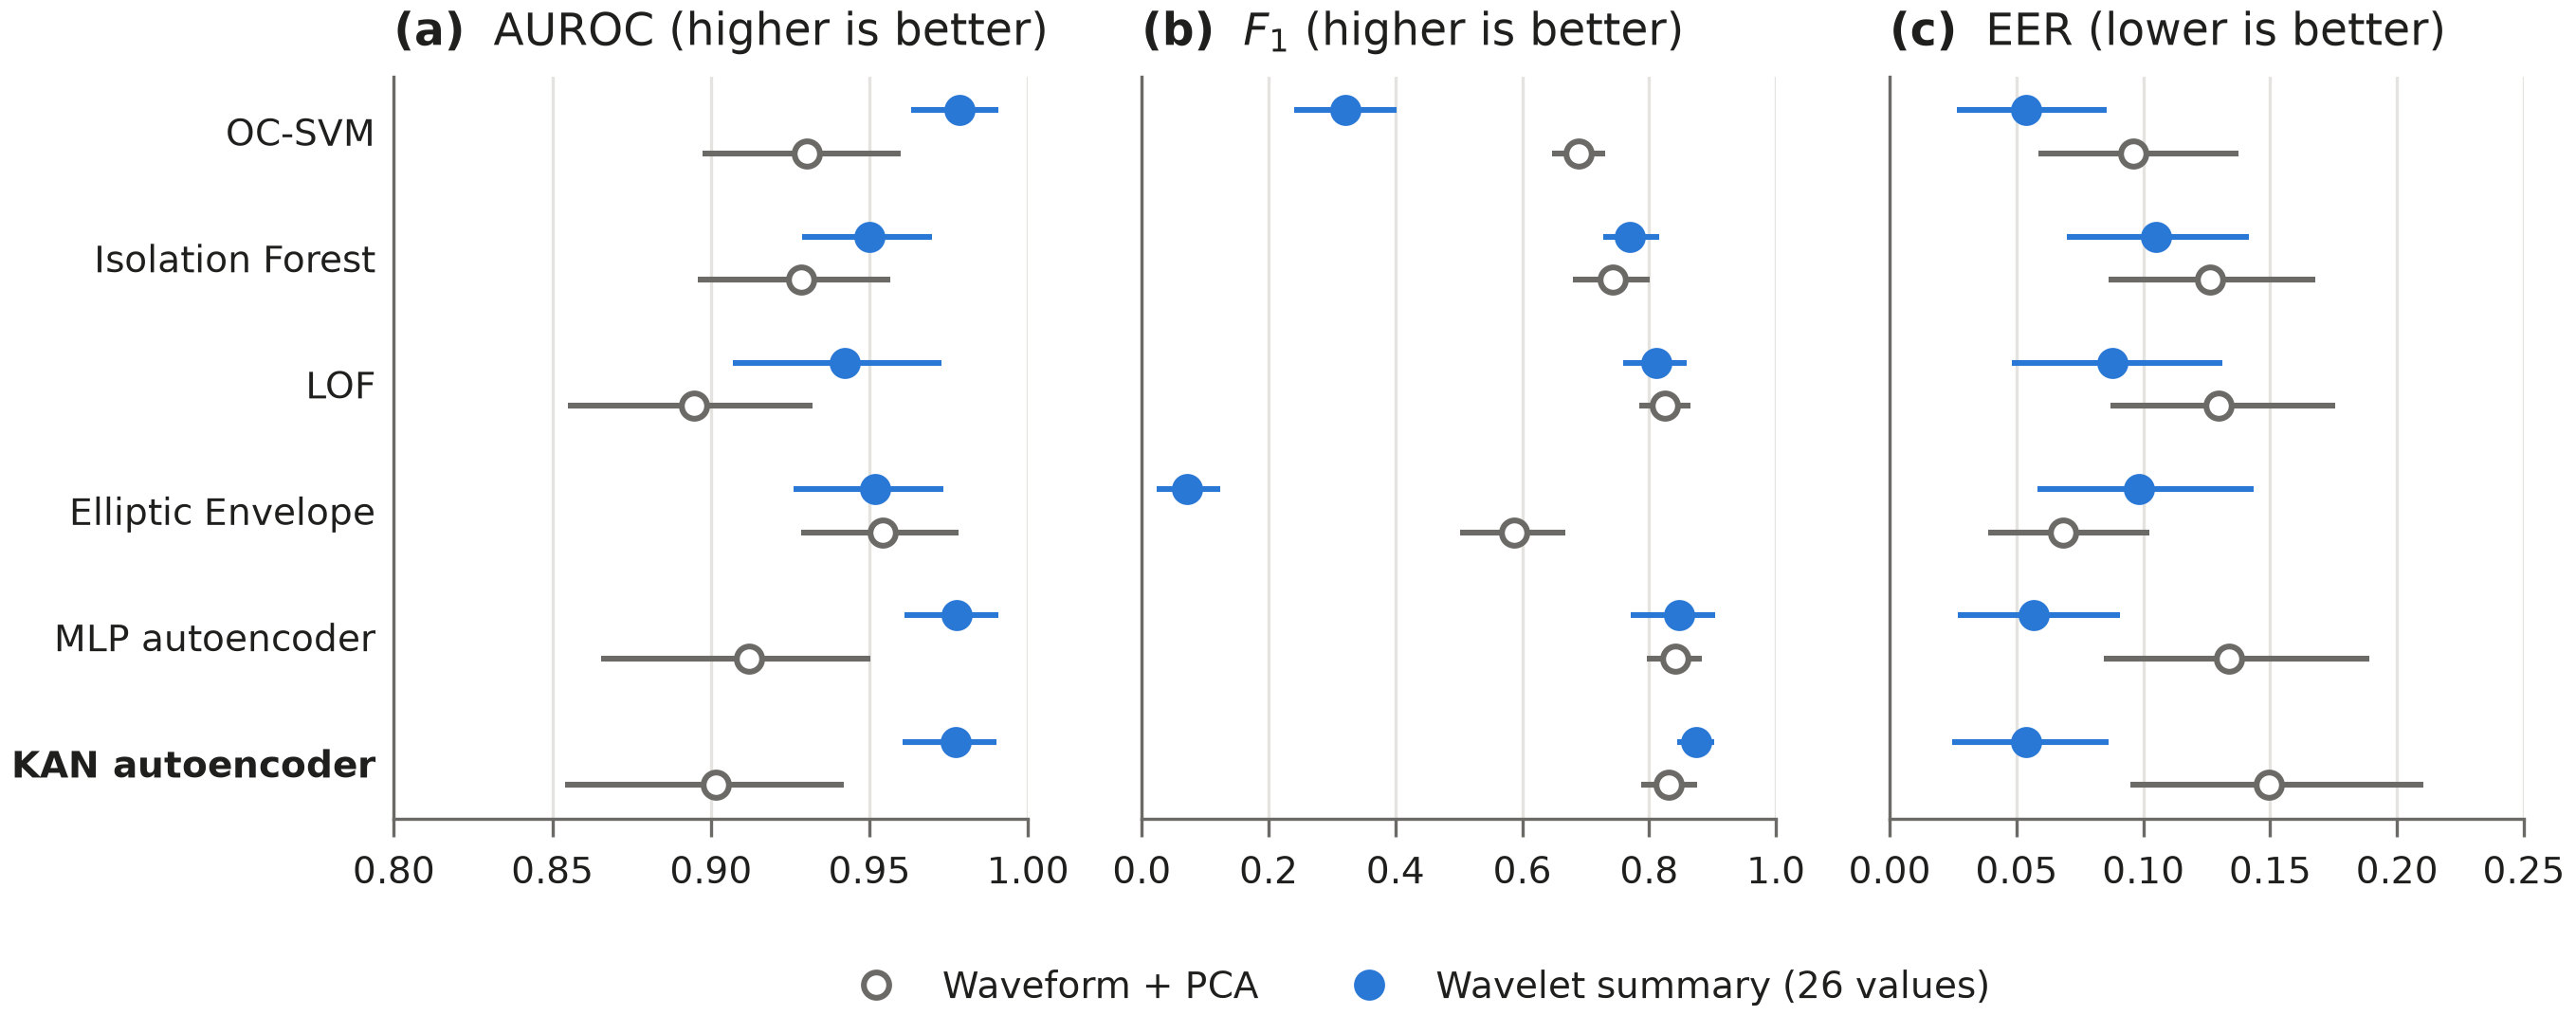
\includegraphics[width=\textwidth]{fig_bars.png}
\caption{Mean performance over 30 participants for the waveform input
(open grey circles) and the wavelet summary (filled blue circles). Horizontal
lines show 95\% participant-bootstrap intervals. $F_1$ is computed at the
enrolment threshold; AUROC and EER do not depend on it. Note the different
horizontal ranges of the three panels.}
\label{fig:bars}
\end{figure}
\begin{table}[htbp]\centering
\caption{Main test: enrolment and test beats from \texttt{rec\_1} for 30
people. Mean $\pm$ standard deviation over participants, with 95\%
participant-bootstrap intervals in brackets. Bold marks the best rounded mean
for each input type and does not imply a statistically supported advantage.
All models have 30 valid participant results.}
\label{tab:primary}\small\setlength{\tabcolsep}{3pt}
% BEGIN GENERATED TABLE: primary.tex
% Generated by research/build_paper_tables.py; do not edit.
\begin{tabular*}{\textwidth}{@{\extracolsep{\fill}}llll@{}}\toprule
Model & AUROC & $F_1$ & EER \\\midrule
\multicolumn{4}{l}{\textit{Waveform with enrolment-fitted PCA}} \\[3pt]
OC-SVM & \shortstack[l]{0.930$\pm$0.091\\[.2ex]{}[0.897, 0.960]} & \shortstack[l]{0.689$\pm$0.119\\[.2ex]{}[0.647, 0.730]} & \shortstack[l]{0.096$\pm$0.113\\[.2ex]{}[0.059, 0.137]} \\[3pt]
Isolation Forest & \shortstack[l]{0.928$\pm$0.087\\[.2ex]{}[0.896, 0.957]} & \shortstack[l]{0.742$\pm$0.173\\[.2ex]{}[0.679, 0.800]} & \shortstack[l]{0.126$\pm$0.117\\[.2ex]{}[0.086, 0.168]} \\[3pt]
LOF & \shortstack[l]{0.895$\pm$0.111\\[.2ex]{}[0.855, 0.932]} & \shortstack[l]{0.825$\pm$0.115\\[.2ex]{}[0.784, 0.865]} & \shortstack[l]{0.130$\pm$0.126\\[.2ex]{}[0.087, 0.176]} \\[3pt]
Elliptic Envelope & \shortstack[l]{\textbf{0.954}$\pm$0.072\\[.2ex]{}[0.928, 0.978]} & \shortstack[l]{0.587$\pm$0.239\\[.2ex]{}[0.502, 0.668]} & \shortstack[l]{\textbf{0.069}$\pm$0.090\\[.2ex]{}[0.039, 0.102]} \\[3pt]
MLP autoencoder & \shortstack[l]{0.912$\pm$0.121\\[.2ex]{}[0.866, 0.950]} & \shortstack[l]{\textbf{0.841}$\pm$0.122\\[.2ex]{}[0.797, 0.883]} & \shortstack[l]{0.134$\pm$0.151\\[.2ex]{}[0.085, 0.189]} \\[3pt]
KAN autoencoder & \shortstack[l]{0.901$\pm$0.126\\[.2ex]{}[0.854, 0.942]} & \shortstack[l]{0.832$\pm$0.124\\[.2ex]{}[0.788, 0.875]} & \shortstack[l]{0.149$\pm$0.163\\[.2ex]{}[0.095, 0.210]} \\[3pt]
\midrule
\multicolumn{4}{l}{\textit{WTMM-inspired summary (26 features)}} \\[3pt]
OC-SVM & \shortstack[l]{\textbf{0.979}$\pm$0.039\\[.2ex]{}[0.963, 0.991]} & \shortstack[l]{0.321$\pm$0.228\\[.2ex]{}[0.241, 0.401]} & \shortstack[l]{\textbf{0.054}$\pm$0.083\\[.2ex]{}[0.027, 0.086]} \\[3pt]
Isolation Forest & \shortstack[l]{0.950$\pm$0.058\\[.2ex]{}[0.929, 0.970]} & \shortstack[l]{0.770$\pm$0.124\\[.2ex]{}[0.728, 0.816]} & \shortstack[l]{0.105$\pm$0.101\\[.2ex]{}[0.070, 0.142]} \\[3pt]
LOF & \shortstack[l]{0.942$\pm$0.095\\[.2ex]{}[0.907, 0.973]} & \shortstack[l]{0.811$\pm$0.143\\[.2ex]{}[0.759, 0.860]} & \shortstack[l]{0.088$\pm$0.121\\[.2ex]{}[0.048, 0.131]} \\[3pt]
Elliptic Envelope & \shortstack[l]{0.952$\pm$0.068\\[.2ex]{}[0.926, 0.973]} & \shortstack[l]{0.071$\pm$0.141\\[.2ex]{}[0.024, 0.124]} & \shortstack[l]{0.098$\pm$0.120\\[.2ex]{}[0.058, 0.143]} \\[3pt]
MLP autoencoder & \shortstack[l]{0.977$\pm$0.043\\[.2ex]{}[0.961, 0.991]} & \shortstack[l]{0.848$\pm$0.190\\[.2ex]{}[0.772, 0.905]} & \shortstack[l]{0.057$\pm$0.092\\[.2ex]{}[0.027, 0.091]} \\[3pt]
KAN autoencoder & \shortstack[l]{0.977$\pm$0.042\\[.2ex]{}[0.961, 0.990]} & \shortstack[l]{\textbf{0.875}$\pm$0.083\\[.2ex]{}[0.845, 0.903]} & \shortstack[l]{\textbf{0.054}$\pm$0.087\\[.2ex]{}[0.025, 0.086]} \\[3pt]
\bottomrule\end{tabular*}
% END GENERATED TABLE: primary.tex
\end{table}

\subsection{Comparison of the leading models}
On the wavelet input, OC-SVM, the MLP and the KAN had almost identical means:
AUROC 0.979, 0.977 and 0.977, and EER 0.054, 0.057 and 0.054. The paired
intervals in Table~\ref{tab:paired} confirm that the data cannot distinguish
the KAN from either model on these two measures. For the two autoencoders,
the agreement holds person by person (Fig.~\ref{fig:perperson}a): the KAN and
the MLP gave exactly the same AUROC for 27 of the 30 participants, 19 of them
at 1.00, and the same EER for 29. The positive paired EER interval in
Table~\ref{tab:paired}, whose lower bound is 0.0000, comes from the single
participant whose EER differed and should not be read as evidence of an
advantage.

The KAN had the highest mean $F_1$ (0.875) and the smallest spread across
participants (standard deviation 0.083). Its mean advantage over the MLP was
0.027, but the paired interval ($-0.020$ to 0.094) includes zero, and
Fig.~\ref{fig:perperson}b shows why: $F_1$ was higher for the KAN in five
participants, higher for the MLP in five, and equal in the remaining 20. The
mean difference is driven largely by one participant for whom the MLP accepted
no genuine probe.

Against Isolation Forest, LOF and Elliptic Envelope, the paired intervals of
the KAN exclude zero for all three measures. These comparisons are
encouraging, but they include development participants and were not corrected
for multiple testing.
\begin{table}[htbp]\centering
\caption{Paired differences between the KAN autoencoder and each other model
on the wavelet summary: KAN minus comparator for AUROC and $F_1$, comparator
minus KAN for EER, so that positive values favour the KAN. Brackets give 95\%
intervals from resampling participants' paired differences.}
\label{tab:paired}\small\setlength{\tabcolsep}{3pt}
% BEGIN GENERATED TABLE: paired.tex
% Generated by research/build_paper_tables.py; do not edit.
\begin{tabular*}{\textwidth}{@{\extracolsep{\fill}}llll@{}}\toprule
Baseline & AUROC & $F_1$ & EER \\\midrule
MLP autoencoder & \shortstack[l]{$-0.0003$\\[.2ex]{}[$-0.0038$, $0.0025$]} & \shortstack[l]{$+0.0268$\\[.2ex]{}[$-0.0199$, $0.0936$]} & \shortstack[l]{$+0.0028$\\[.2ex]{}[$0.0000$, $0.0083$]} \\[3pt]
OC-SVM & \shortstack[l]{$-0.0014$\\[.2ex]{}[$-0.0059$, $0.0028$]} & \shortstack[l]{$+0.5541$\\[.2ex]{}[$0.4711$, $0.6375$]} & \shortstack[l]{$-0.0003$\\[.2ex]{}[$-0.0167$, $0.0181$]} \\[3pt]
Isolation Forest & \shortstack[l]{$+0.0272$\\[.2ex]{}[$0.0150$, $0.0403$]} & \shortstack[l]{$+0.1046$\\[.2ex]{}[$0.0548$, $0.1524$]} & \shortstack[l]{$+0.0509$\\[.2ex]{}[$0.0224$, $0.0830$]} \\[3pt]
LOF & \shortstack[l]{$+0.0348$\\[.2ex]{}[$0.0111$, $0.0624$]} & \shortstack[l]{$+0.0634$\\[.2ex]{}[$0.0203$, $0.1132$]} & \shortstack[l]{$+0.0337$\\[.2ex]{}[$0.0061$, $0.0645$]} \\[3pt]
Elliptic Envelope & \shortstack[l]{$+0.0252$\\[.2ex]{}[$0.0074$, $0.0481$]} & \shortstack[l]{$+0.8041$\\[.2ex]{}[$0.7493$, $0.8552$]} & \shortstack[l]{$+0.0445$\\[.2ex]{}[$0.0013$, $0.0910$]} \\[3pt]
\bottomrule\end{tabular*}
% END GENERATED TABLE: paired.tex
\end{table}
\begin{figure}[htbp]\centering
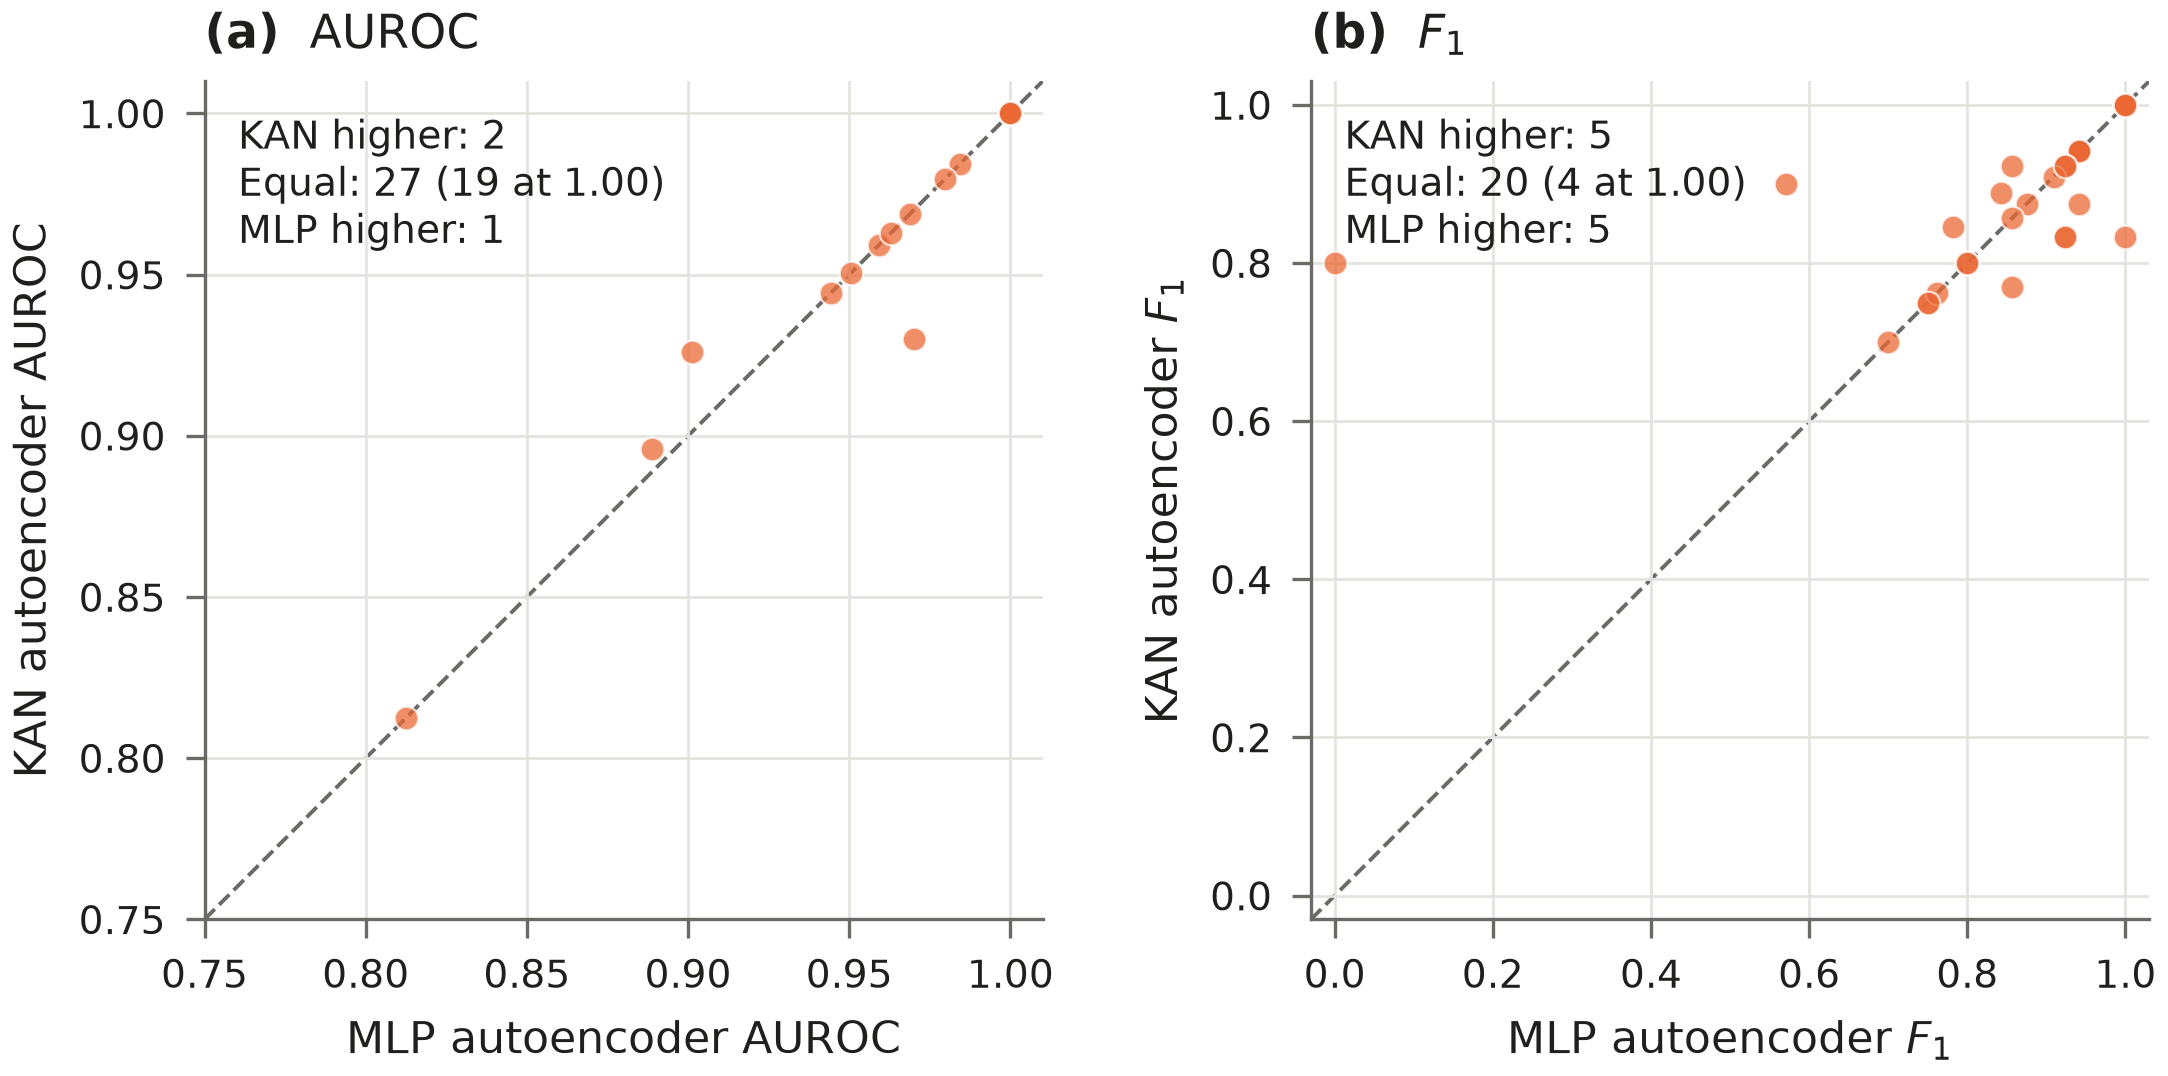
\includegraphics[width=0.8\textwidth]{fig_perperson.png}
\caption{Per-participant comparison of the KAN and MLP autoencoders on the
wavelet summary. Each point is one participant; points on the dashed line
indicate equal values. (a)~AUROC. (b)~$F_1$ at the enrolment threshold.}
\label{fig:perperson}
\end{figure}

OC-SVM and Elliptic Envelope ranked the probes well but had low $F_1$
(0.321 and 0.071). The balanced probe sets allow the cause to be identified.
If a person has equally many genuine and impostor probes and a fraction $R$ of
the genuine probes is accepted, precision cannot fall below $R/(1+R)$, so
$F_1\ge 2R/(2+R)$, or equivalently $R\le 2F_1/(2-F_1)$. Applying this bound to
each participant and averaging shows that Elliptic Envelope accepted, on
average, no more than 9\% of genuine probes and OC-SVM no more than 43\%. The low $F_1$ of these two models
therefore reflects genuine beats being rejected by an over-tight enrolment
threshold, not impostors being accepted. Enrolment beats from the same
recording appear to receive systematically better scores than new beats from
the same person, which the minimum-score rule cannot absorb. Calibrating the
threshold on held-out enrolment beats could address this without using test
labels, but we did not test it.

\subsection{Differences between participants}
Figure~\ref{fig:heatmap} shows the AUROC of every model for every
participant. With the waveform input, 57 of the 180 model--participant
results fell below 0.90; with the wavelet summary, 23 did. Difficulty was
shared across models: Persons~13, 14 and 21 had low AUROC for most models on
the waveform input, and Person~21 remained the hardest case with the wavelet
summary, where all six models stayed at or below 0.81. Recording quality or
beat-to-beat variability may contribute, but these data do not establish the
cause. Many participants had an AUROC of exactly 1.00 (19 for the KAN with the
wavelet summary). Given only 6--12 genuine and as many impostor probes, this
means perfect ranking of a small test set, not error-free verification.
\begin{figure}[htbp]\centering
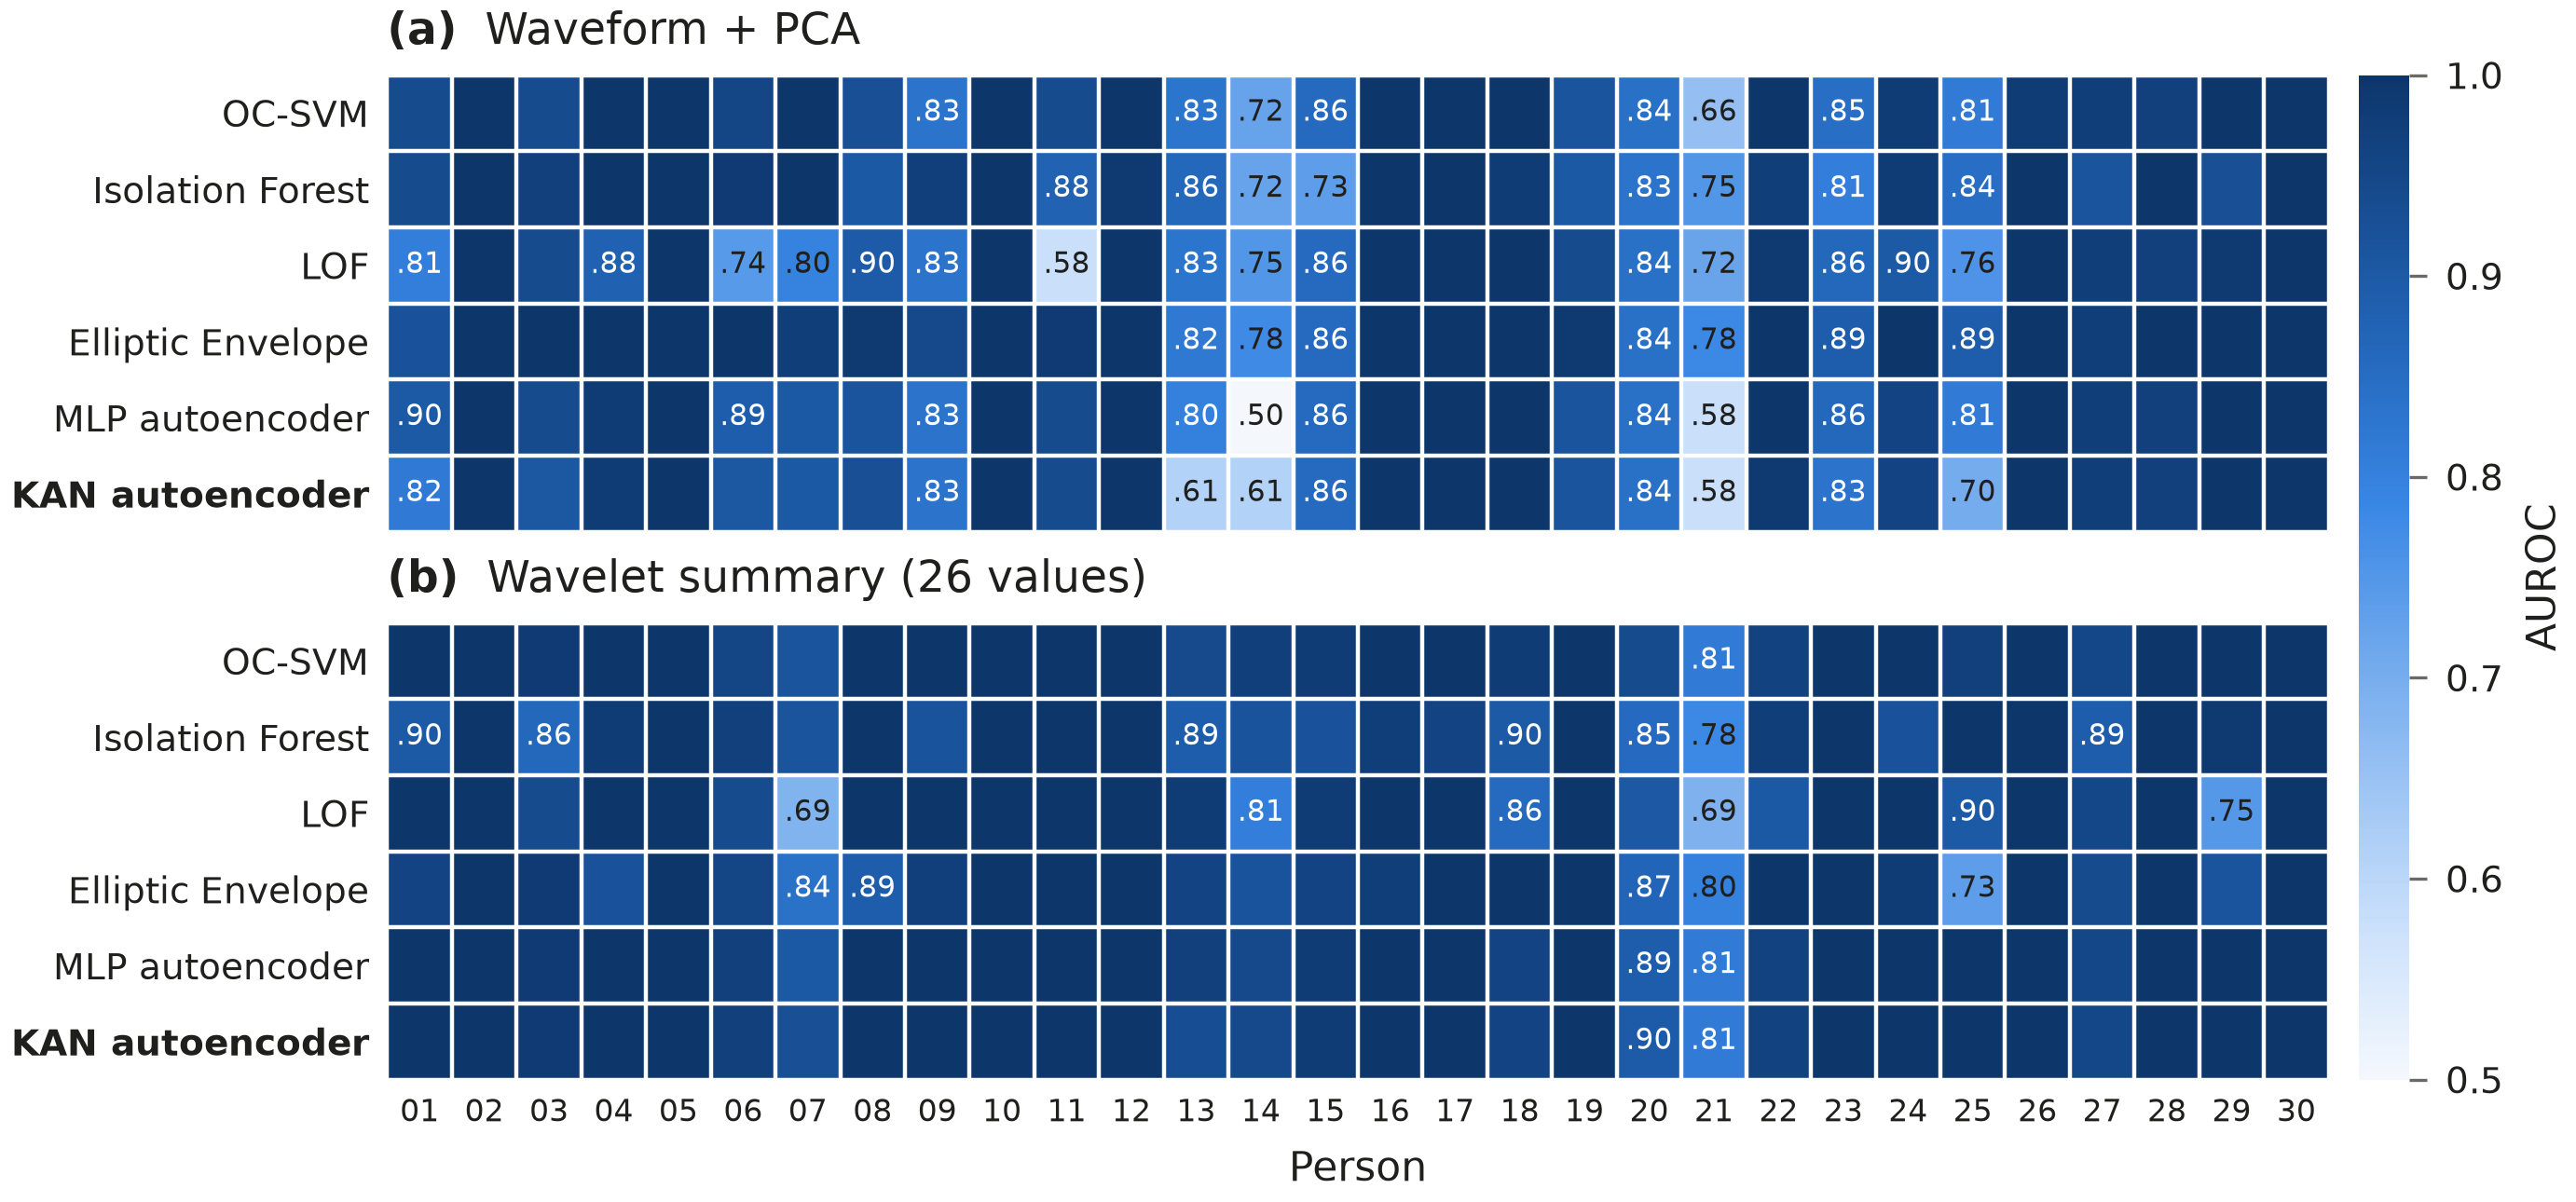
\includegraphics[width=\textwidth]{fig_heatmap.png}
\caption{AUROC for every participant (columns) and model (rows) with
(a)~the waveform input and (b)~the wavelet summary. Darker cells are better;
values are printed only where AUROC is below 0.90.}\label{fig:heatmap}
\end{figure}

Figure~\ref{fig:roc} shows the ROC curves of the two autoencoders, whose
per-probe scores were saved; scores of the classical detectors were not
retained in the original runs. For both networks, the averaged curve of the
wavelet summary lies above that of the waveform input at every false
acceptance rate. For 19 of the 30 participants, each autoencoder accepted
every genuine probe before accepting any impostor.
\begin{figure}[htbp]\centering
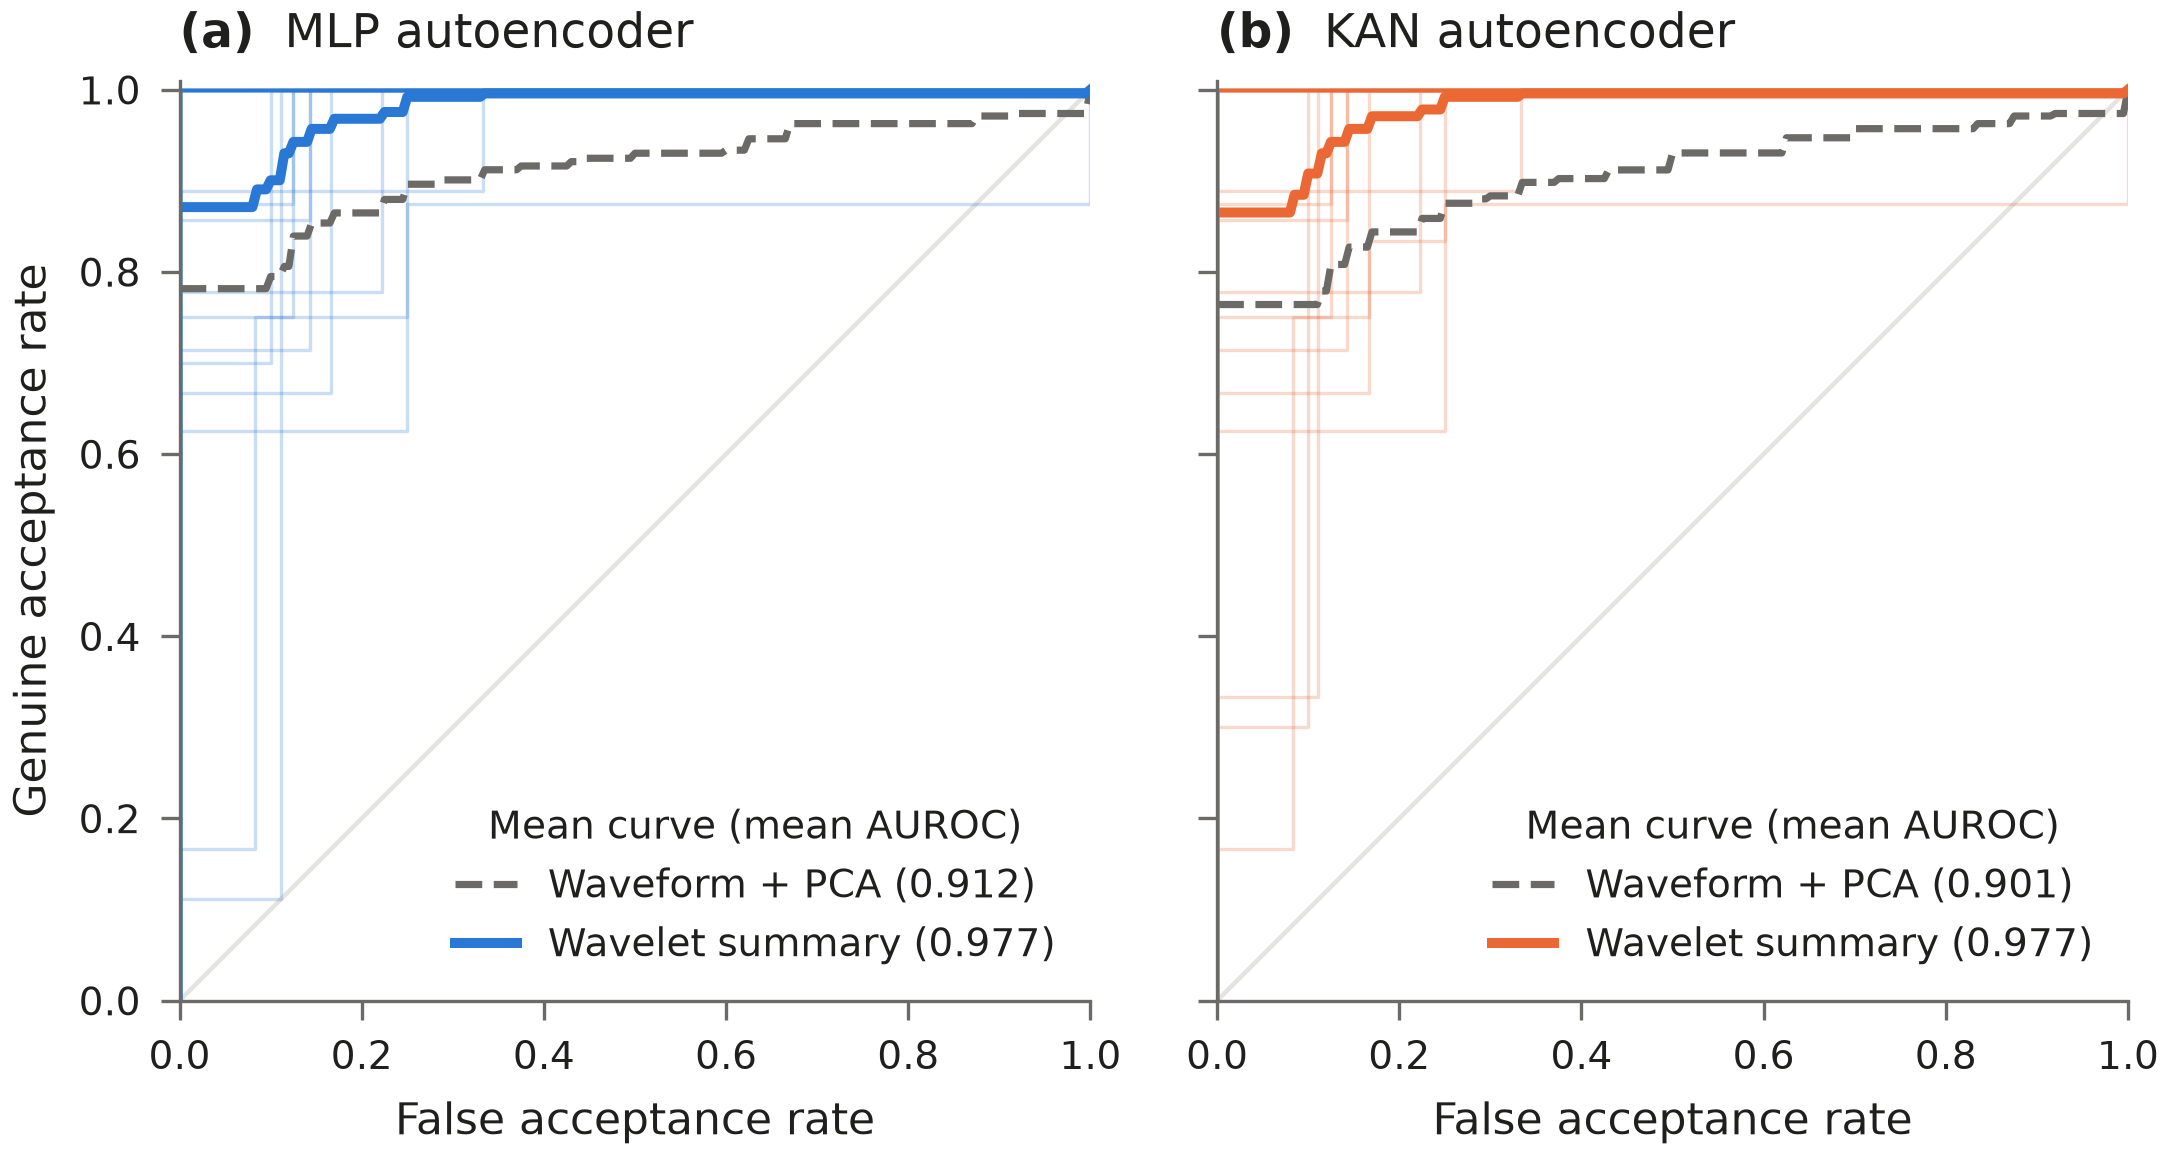
\includegraphics[width=0.8\textwidth]{fig_roc.png}
\caption{ROC curves of (a)~the MLP and (b)~the KAN autoencoder. Thin lines are
individual participants with the wavelet summary; thick lines are vertical
averages over the 30 participants for each input. Legend values are mean
per-participant AUROCs.}\label{fig:roc}
\end{figure}

\FloatBarrier
\subsection{Testing on a second recording}\label{sec:cross}
Table~\ref{tab:cross} gives the results for ten participants enrolled on
\texttt{rec\_1} and tested on \texttt{rec\_2}. With the Gaussian-derivative
wavelet, the KAN reached AUROC 0.938, $F_1$ 0.670 and EER 0.106; with the
Morlet wavelet, 0.952, 0.711 and 0.086. The Morlet means are better, but no
paired comparison between the wavelets was made, and both runs use the same
development participants.

Among the leading models with Morlet features, the KAN had the highest mean
$F_1$ and the lowest mean EER, whereas OC-SVM had the highest AUROC. These
differences are small relative to the intervals, and overlapping intervals
cannot substitute for a paired analysis.
\begin{table}[htbp]\centering
\caption{Second-recording test on Persons~01--10: enrolment on all usable
\texttt{rec\_1} beats, testing on \texttt{rec\_2}. Means over participants
with 95\% participant-bootstrap intervals. Bold marks the best rounded mean
among the six models for each wavelet. Every model has ten valid participant
results.}
\label{tab:cross}\small\setlength{\tabcolsep}{4pt}
% BEGIN GENERATED TABLE: second_recording.tex
% Generated by research/build_paper_tables.py; do not edit.
\begin{tabular*}{\textwidth}{@{\extracolsep{\fill}}llll@{}}\toprule
Model & AUROC & $F_1$ & EER \\\midrule
\multicolumn{4}{l}{\textit{Gaussian derivative}} \\[3pt]
OC-SVM & \shortstack[l]{0.940\\[.2ex]{}[0.892, 0.972]} & \shortstack[l]{0.222\\[.2ex]{}[0.076, 0.372]} & \shortstack[l]{\textbf{0.098}\\[.2ex]{}[0.047, 0.164]} \\[3pt]
Isolation Forest & \shortstack[l]{0.896\\[.2ex]{}[0.807, 0.959]} & \shortstack[l]{0.667\\[.2ex]{}[0.518, 0.767]} & \shortstack[l]{0.147\\[.2ex]{}[0.079, 0.243]} \\[3pt]
LOF & \shortstack[l]{0.934\\[.2ex]{}[0.888, 0.964]} & \shortstack[l]{0.668\\[.2ex]{}[0.458, 0.840]} & \shortstack[l]{0.128\\[.2ex]{}[0.075, 0.190]} \\[3pt]
Elliptic Envelope & \shortstack[l]{0.913\\[.2ex]{}[0.860, 0.956]} & \shortstack[l]{0.074\\[.2ex]{}[0.000, 0.222]} & \shortstack[l]{0.143\\[.2ex]{}[0.085, 0.217]} \\[3pt]
MLP autoencoder & \shortstack[l]{\textbf{0.946}\\[.2ex]{}[0.917, 0.968]} & \shortstack[l]{\textbf{0.671}\\[.2ex]{}[0.454, 0.852]} & \shortstack[l]{0.118\\[.2ex]{}[0.072, 0.168]} \\[3pt]
KAN autoencoder & \shortstack[l]{0.938\\[.2ex]{}[0.891, 0.970]} & \shortstack[l]{0.670\\[.2ex]{}[0.450, 0.856]} & \shortstack[l]{0.106\\[.2ex]{}[0.059, 0.154]} \\[3pt]
\midrule
\multicolumn{4}{l}{\textit{Morlet}} \\[3pt]
OC-SVM & \shortstack[l]{\textbf{0.955}\\[.2ex]{}[0.922, 0.981]} & \shortstack[l]{0.248\\[.2ex]{}[0.118, 0.382]} & \shortstack[l]{0.103\\[.2ex]{}[0.054, 0.155]} \\[3pt]
Isolation Forest & \shortstack[l]{0.889\\[.2ex]{}[0.820, 0.949]} & \shortstack[l]{0.640\\[.2ex]{}[0.480, 0.747]} & \shortstack[l]{0.164\\[.2ex]{}[0.103, 0.225]} \\[3pt]
LOF & \shortstack[l]{0.943\\[.2ex]{}[0.915, 0.971]} & \shortstack[l]{0.692\\[.2ex]{}[0.484, 0.860]} & \shortstack[l]{0.101\\[.2ex]{}[0.056, 0.145]} \\[3pt]
Elliptic Envelope & \shortstack[l]{0.921\\[.2ex]{}[0.873, 0.962]} & \shortstack[l]{0.075\\[.2ex]{}[0.000, 0.206]} & \shortstack[l]{0.136\\[.2ex]{}[0.078, 0.203]} \\[3pt]
MLP autoencoder & \shortstack[l]{0.953\\[.2ex]{}[0.922, 0.980]} & \shortstack[l]{0.701\\[.2ex]{}[0.488, 0.868]} & \shortstack[l]{0.090\\[.2ex]{}[0.046, 0.137]} \\[3pt]
KAN autoencoder & \shortstack[l]{0.952\\[.2ex]{}[0.920, 0.978]} & \shortstack[l]{\textbf{0.711}\\[.2ex]{}[0.489, 0.884]} & \shortstack[l]{\textbf{0.086}\\[.2ex]{}[0.047, 0.128]} \\[3pt]
\bottomrule\end{tabular*}
% END GENERATED TABLE: second_recording.tex
\end{table}

The leading models scored lower here than in the main test, and $F_1$ in
particular dropped to about 0.7 for the autoencoders. A plausible reason is
that beats from a new recording differ more from the enrolment beats than
held-out beats from the same recording do, so more genuine beats exceed the
enrolment threshold. The two tests also differ in participants, enrolment
size and impostor pool, however, so isolating the effect of the recording
would require both protocols to be run on the same people under otherwise
matched conditions.

\subsection{Results by participant group}
Table~\ref{tab:cohorts} splits the main wavelet results into Persons~01--10
and Persons~11--30, using the same per-person results rather than new models.
The KAN reached a mean AUROC of 0.988 in the first group and 0.972 in the
second, and the three leading models stayed close to one another in both. As
the groups share one training run and impostor pool, and the design
comparison covered both, the split is descriptive and does not constitute
independent validation.
\begin{table}[htbp]\centering
\caption{Mean results of the main Gaussian-wavelet test by participant
group. Both groups may have influenced model development.}
\label{tab:cohorts}\small
% BEGIN GENERATED TABLE: cohorts.tex
% Generated by research/build_paper_tables.py; do not edit.
\begin{tabular}{lllll}\toprule
Persons & Model & AUROC & $F_1$ & EER \\\midrule
01--10 & OC-SVM & 0.985 & 0.365 & 0.024 \\
01--10 & MLP autoencoder & 0.985 & 0.822 & 0.037 \\
01--10 & KAN autoencoder & 0.988 & 0.877 & 0.037 \\
11--30 & OC-SVM & 0.975 & 0.298 & 0.068 \\
11--30 & MLP autoencoder & 0.973 & 0.861 & 0.067 \\
11--30 & KAN autoencoder & 0.972 & 0.873 & 0.062 \\
\bottomrule\end{tabular}
% END GENERATED TABLE: cohorts.tex
\end{table}

\FloatBarrier
\section{Discussion}\label{sec:discussion}
\subsection{What the wavelet comparison shows}
The wavelet summary improved AUROC for five of the six models, which suggests
that it captures identity information in a form these one-class models can
exploit with few enrolment beats. This does not imply that the waveform lacks
such information. After PCA the waveform input has at most 26 informative
dimensions, and it is normalised per beat, whereas the wavelet summary keeps
amplitude. A controlled follow-up should equalise the normalisation and vary
one factor at a time.

Figure~\ref{fig:tsne} projects all 747 beats of the main test into two
dimensions with t-SNE \cite{maaten2008} (features standardised over all
participants, PCA initialisation, perplexity 30, seed 42). Note that the
waveform panel uses the full standardised 350-sample beats, not the
enrolment-fitted PCA inputs of the verifiers. Perhaps surprisingly, many
participants form tighter and better separated groups in the waveform view
than in the wavelet view, although the wavelet input gave the higher
verification AUROC. Person~01 illustrates the opposite pattern: its beats are
split among several groups in the waveform view but form one compact group in
the wavelet view. Persons~14 and 21, both difficult cases in
Fig.~\ref{fig:heatmap}, are dispersed in both views. A global map of all
participants is not the decision each verifier makes, which compares a single
person's enrolment beats with new beats, so the figure illustrates the data
but cannot explain the AUROC difference.
\begin{figure}[htbp]\centering
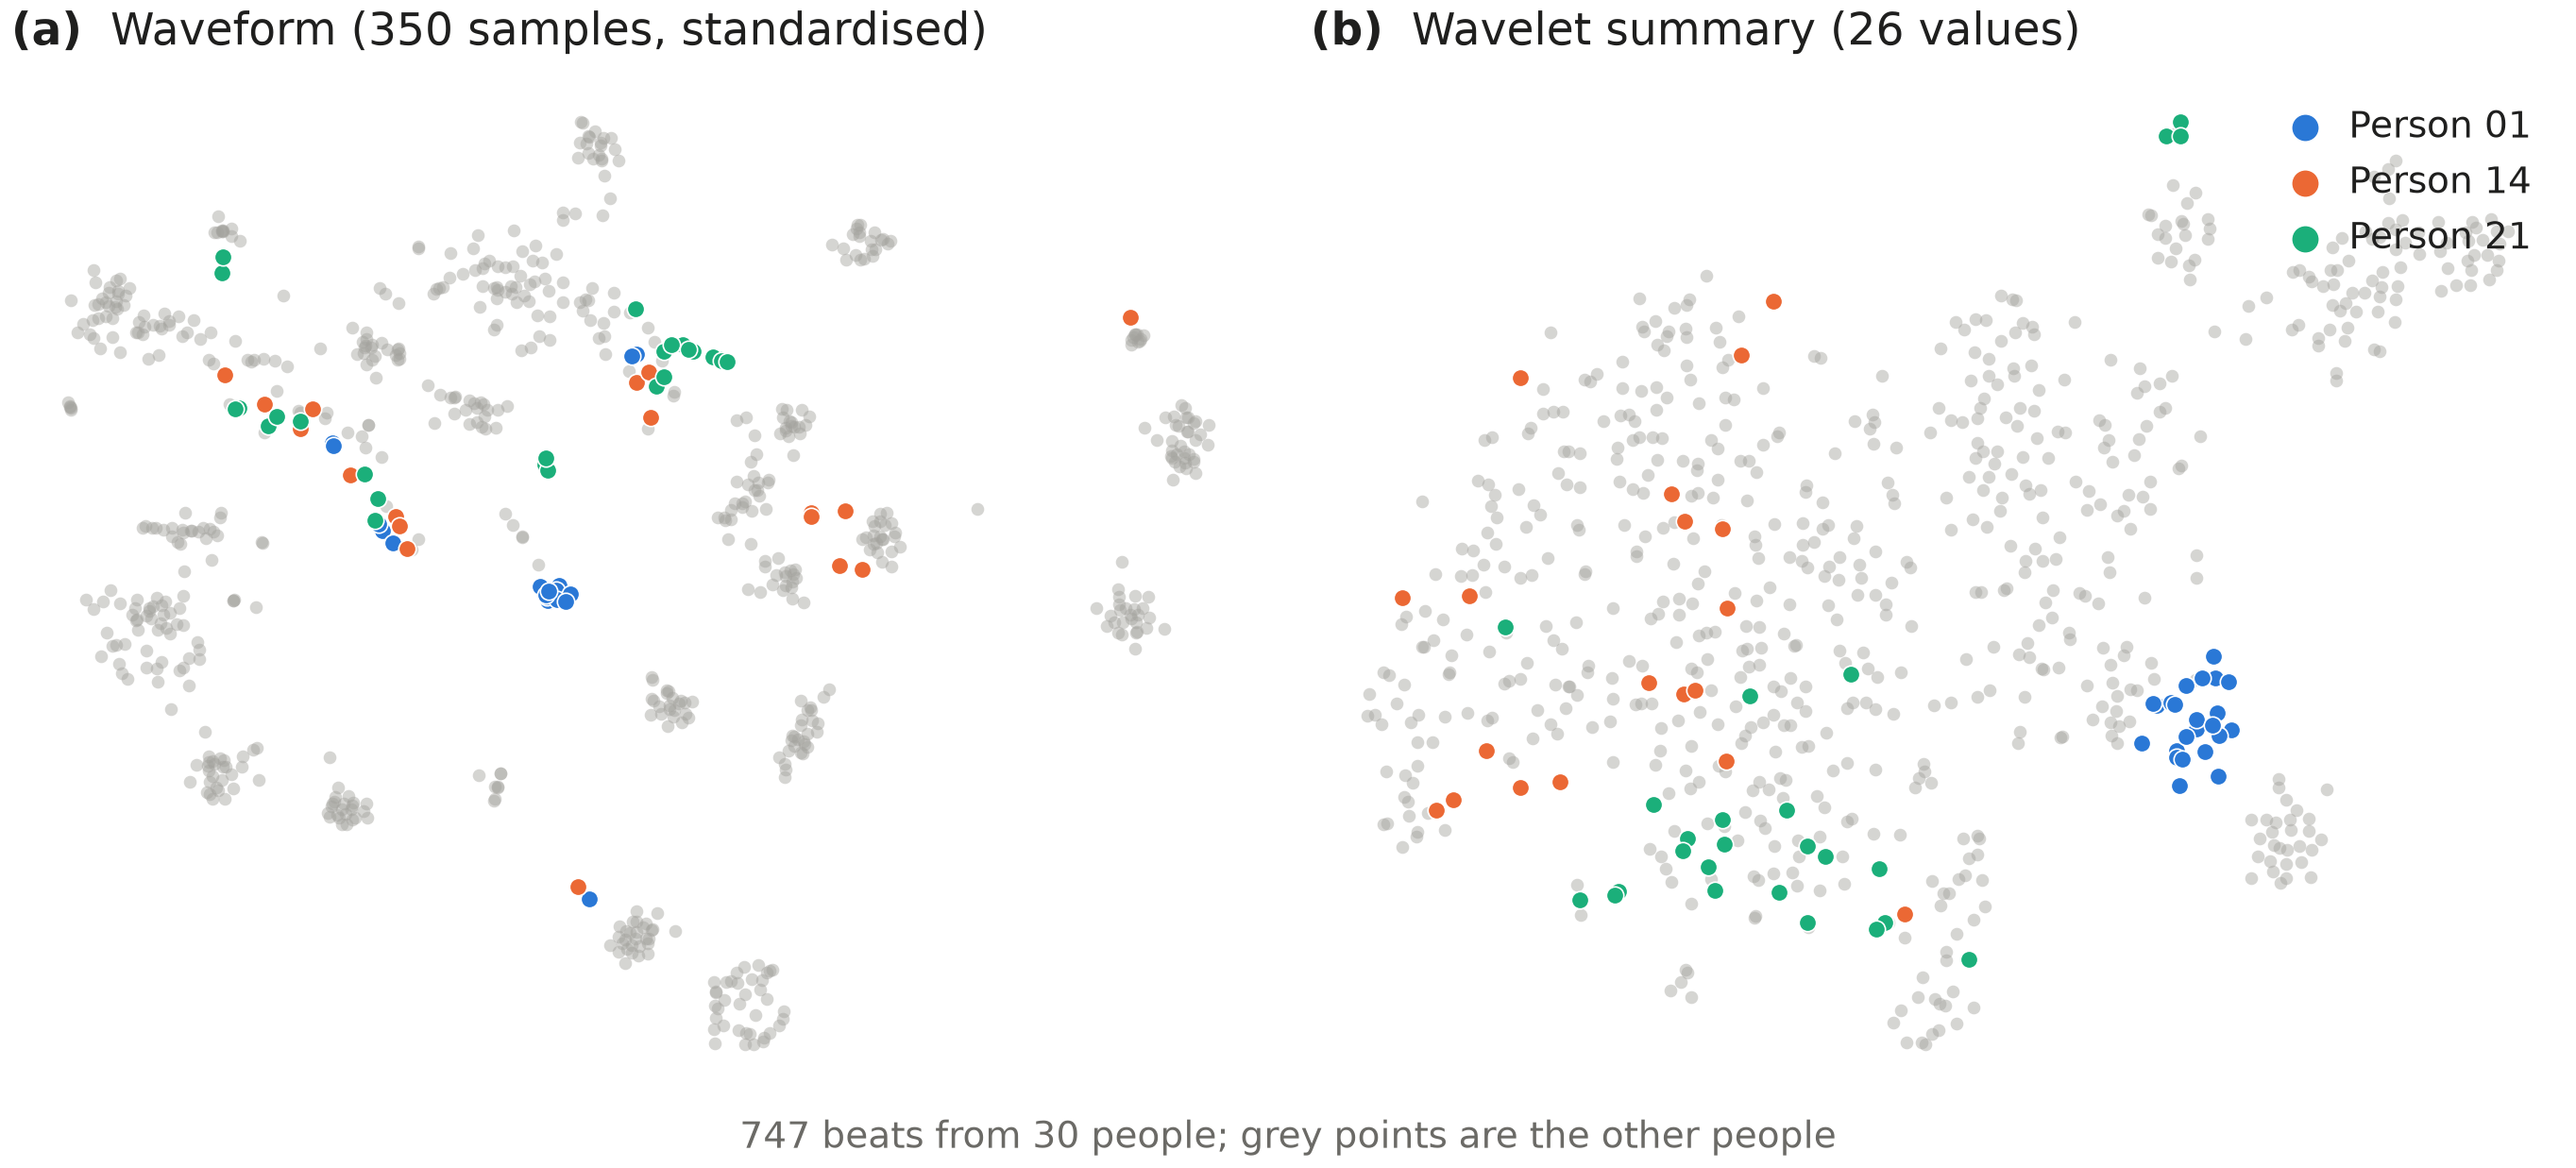
\includegraphics[width=\textwidth]{fig_tsne.png}
\caption{Two-dimensional t-SNE views of the 747 main-test beats using
(a)~standardised 350-sample waveforms and (b)~the 26-value wavelet summary.
Three participants are highlighted; all other beats are shown in grey. The
cluster structure is illustrative and should not be used to rank the two
inputs.}
\label{fig:tsne}
\end{figure}

\subsection{What the KAN comparison shows}
The KAN autoencoder matched the ranking performance of the MLP autoencoder
with 39\% of its parameters, and in most participants the two produced
identical AUROC and EER. Its higher mean $F_1$ is not supported by the paired
analysis. The evidence therefore supports the KAN as a compact alternative
for this task, not as a more accurate or faster model.

The two networks differ in width, code size, edge functions and the effort
spent on choosing their settings, so parameter count alone cannot attribute
the result to the KAN design \cite{yu2024}. Inference time and energy should
be measured on a specified device before any deployment advantage is claimed.
Nor do we claim that the learned splines are physiologically interpretable;
this was not examined.

\subsection{Relation to other ECG biometric studies}
Identification selects one identity among those learned during training,
whereas verification tests a single claim. Our verifiers see only the
claimant's genuine beats. Identification accuracies reported in earlier work
\cite{byeon2019,elboujnouni2022,elboujnouni2020} are therefore not directly
comparable with our AUROC, EER or $F_1$. ECGXtractor \cite{melzi2022} does
address verification, but it learns its representation from a large external
population and aggregates several beats, so its EER is not a matched baseline
for per-person, single-beat verification. Clinical ECG classification
\cite{ozaltin2023} addresses a different question altogether.

\subsection{Limitations and future work}
The evidence comes from small samples. The main test covers 30 people with
one recording each, and the second test ten development participants with two
same-day recordings. The saved design comparison includes both participant
groups, the MLP received less tuning than the KAN, and no dated record of the
selection process exists. Neither experiment therefore measures performance
on people who were unseen during development, or on recordings from a later
day.

Most results come from a single run seed, and a different seed or processing
order would change the neural training sequence; repeated runs are needed,
particularly because the leading AUROC means differ only in the third
decimal. With 6--12 genuine probes per person, individual estimates are
coarse. Impostor pools are shared across people, and the participant
bootstrap does not cover every source of variation.

Several methodological limits also apply. Beat windows from the same
recording may overlap, and cleaning operates on the whole recording. The
Elliptic Envelope covariance can be unstable with few beats, the lowest
wavelet frequencies are affected by the window edges, and the two inputs are
normalised differently. The minimum-score threshold has not been compared
with other enrolment-only calibration methods, and no external cohort,
post-exercise data or spoofing attacks were tested.

A confirmatory study should fix all settings in advance, evaluate
participants who played no part in development, repeat training over several
seeds, compare recordings within the same people, match normalisation between
the inputs, report all failed runs and measure efficiency on target hardware.

\section{Conclusion}\label{sec:conclusion}
We studied ECG verification with a short enrolment recording and no impostor
training data. A 26-value summary of wavelet maxima ridges raised the mean
AUROC of five of six one-class models, for example from 0.930 to 0.979 for
OC-SVM and from 0.912 to 0.977 for an MLP autoencoder.

A compact KAN autoencoder reached a mean AUROC of 0.977 and an EER of 0.054
with 3{,}248 parameters, against 8{,}422 for the MLP, and its ranking
performance was indistinguishable from that of the MLP and OC-SVM in paired
comparisons. It had the highest mean $F_1$ at the enrolment threshold, but
its advantage over the MLP was not clear. Two classical detectors lost most
of their $F_1$ because the enrolment threshold rejected genuine beats, which
makes threshold calibration a priority for future work. Results on a second
same-day recording were lower but remained informative. Taken together, the
findings support compact KAN autoencoders as candidates for further ECG
verification research, pending independent evaluation and better
calibration.

\section*{Declaration of competing interest}
The authors declare that they have no known competing financial interests or
personal relationships that could have appeared to influence the work
reported in this paper.

\section*{Code and data availability}
The manuscript, code and participant-level results are available at
\url{https://github.com/usmhic/ecg-kan}. ECG-ID version 1.0.0 can be obtained
from \url{https://physionet.org/content/ecgiddb/1.0.0/} under the Open Data
Commons Attribution License v1.0; the raw recordings are not redistributed
with the code. The software environment and split manifests of the original
runs were not archived, so exact reproduction of those runs cannot be
guaranteed. The release notes list the evidence that was retained and the
checks that can be repeated.

\section*{Ethics and consent}
This study uses only the public ECG-ID database and involved no new data
collection. Data acquisition and participant information are described by
the database creator \cite{lugovaya2005}.

\section*{Declaration of generative AI and AI-assisted technologies in the
writing process}
The authors designed the study, carried out the experiments and wrote the
original draft. Large language models were later used to help review and
edit the text, improve its clarity, and check the consistency between the
methods description and the code. These tools did not generate or validate
experimental results. The authors reviewed and edited all content and take
full responsibility for the published article.

\begin{thebibliography}{99}
\bibitem{bhuva2023}
D.~R. Bhuva, S.~Kumar, A novel continuous authentication method using biometrics
for IOT devices, Internet of Things 24 (2023) 100927.
\url{https://doi.org/10.1016/j.iot.2023.100927}.
\bibitem{melzi2022}
P.~Melzi, R.~Tolosana, R.~Vera-Rodriguez, ECG biometric recognition: Review,
system proposal, and benchmark evaluation, IEEE Access 11 (2023) 15555--15566.
\bibitem{clifford2006}
G.~D. Clifford, F.~Azuaje, P.~E. McSharry (Eds.), Advanced Methods and Tools
for ECG Data Analysis, Artech House, 2006.
\bibitem{byeon2019}
Y.-H. Byeon, S.-B. Pan, K.-C. Kwak, Intelligent deep models based on scalograms
of electrocardiogram signals for biometrics, Sensors 19 (4) (2019) 935.
\bibitem{mallat1992}
S.~Mallat, W.-L. Hwang, Singularity detection and processing with wavelets,
IEEE Transactions on Information Theory 38 (2) (1992) 617--643.
\bibitem{mallat1999}
S.~Mallat, A Wavelet Tour of Signal Processing, 2nd Edition, Academic Press, 1999.
\bibitem{elboujnouni2022}
I.~El~Boujnouni, H.~Zili, A.~Tali, T.~Tali, Y.~Laaziz, A wavelet-based capsule
neural network for ECG biometric identification, Biomedical Signal Processing
and Control 76 (2022) 103692.
\bibitem{elboujnouni2020}
I.~El~Boujnouni, A.~Tali, K.~Bentaleb, Biometric identification of individuals
based on scalograms of electrocardiogram and capsule network, in: Advanced
Intelligent Systems for Sustainable Development (AI2SD'2020): Volume 2,
Advances in Intelligent Systems and Computing, Vol.~1418, Springer, 2022,
pp.~29--42.
\bibitem{ozaltin2023}
O.~Ozaltin, O.~Yeniay, A novel proposed CNN--SVM architecture for ECG scalograms
classification, Soft Computing 27 (8) (2023) 4639--4658.
\url{https://doi.org/10.1007/s00500-022-07729-x}.
\bibitem{scholkopf2001}
B.~Sch\"olkopf, J.~C. Platt, J.~Shawe-Taylor, A.~J. Smola, R.~C. Williamson,
Estimating the support of a high-dimensional distribution, Neural Computation
13 (7) (2001) 1443--1471.
\bibitem{liu2008}
F.~T. Liu, K.~M. Ting, Z.-H. Zhou, Isolation forest, in: Proceedings of the
IEEE International Conference on Data Mining, 2008, pp.~413--422.
\bibitem{breunig2000}
M.~M. Breunig, H.-P. Kriegel, R.~T. Ng, J.~Sander, LOF: Identifying
density-based local outliers, in: Proceedings of ACM SIGMOD, 2000, pp.~93--104.
\bibitem{tax2004}
D.~M.~J. Tax, R.~P.~W. Duin, Support vector data description, Machine Learning
54 (1) (2004) 45--66.
\bibitem{ruff2021}
L.~Ruff, J.~R. Kauffmann, R.~A. Vandermeulen, G.~Montavon, W.~Samek, M.~Kloft,
T.~G. Dietterich, K.-R. M\"uller, A unifying review of deep and shallow anomaly
detection, Proceedings of the IEEE 109 (5) (2021) 756--795.
\bibitem{kiyasseh2021}
D.~Kiyasseh, T.~Zhu, D.~A. Clifton, CLOCS: Contrastive learning of cardiac
signals across space, time, and patients, in: Proceedings of ICML,
Proceedings of Machine Learning Research 139, 2021, pp.~5606--5615.
\bibitem{liu2024}
Z.~Liu, Y.~Wang, S.~Vaidya, F.~Ruehle, J.~Halverson, M.~Solja\v{c}i\'c,
T.~Y. Hou, M.~Tegmark, KAN: Kolmogorov--Arnold networks, in: Proceedings of
ICLR, 2025. \url{https://arxiv.org/abs/2404.19756}.
\bibitem{yu2024}
R.~Yu, W.~Yu, X.~Wang, KAN or MLP: A fairer comparison, arXiv:2407.16674 (2024).
\bibitem{jahin2025}
M.~A. Jahin, M.~A. Masud, M.~F. Mridha, Z.~Aung, N.~Dey,
KACQ-DCNN: Uncertainty-aware interpretable Kolmogorov--Arnold
classical--quantum dual-channel neural network for heart disease detection,
Computers in Biology and Medicine 197, Part A (2025) 110976.
\url{https://doi.org/10.1016/j.compbiomed.2025.110976}.
\bibitem{zhao2025}
C.~Zhao, B.~Lai, Y.~Xu, Y.~Wang, H.~Dong, MAK-Net: A multi-scale attentive
Kolmogorov--Arnold network with BiGRU for imbalanced ECG arrhythmia
classification, Sensors 25 (13) (2025) 3928.
\url{https://doi.org/10.3390/s25133928}.
\bibitem{moradi2024}
M.~Moradi, S.~Panahi, E.~Bollt, Y.-C. Lai, Kolmogorov--Arnold network
autoencoders, arXiv:2410.02077 (2024).
\url{https://arxiv.org/abs/2410.02077}.
\bibitem{zhou2025kanad}
Q.~Zhou, C.~Pei, F.~Sun, J.~Han, Z.~Gao, D.~Pei, H.~Zhang, G.~Xie, J.~Li,
KAN-AD: Time series anomaly detection with Kolmogorov--Arnold networks,
in: Proceedings of ICML, Proceedings of Machine Learning Research 267,
2025, pp.~79136--79149. \url{https://arxiv.org/abs/2411.00278}.
\bibitem{lomoio2025}
U.~Lomoio, P.~Veltri, P.~H. Guzzi, Kolmogorov Arnold network autoencoder
in medicine, arXiv:2507.19524 (2025).
\url{https://arxiv.org/abs/2507.19524}.
\bibitem{israel2005}
S.~A. Israel, J.~M. Irvine, A.~Cheng, M.~D. Wiederhold, B.~K. Wiederhold,
ECG to identify individuals, Pattern Recognition 38 (1) (2005) 133--142.
\bibitem{pan1985}
J.~Pan, W.~J. Tompkins, A real-time QRS detection algorithm, IEEE Transactions
on Biomedical Engineering BME-32 (3) (1985) 230--236.
\bibitem{makowski2021}
D.~Makowski, T.~Pham, Z.~J. Lau, J.~C. Brammer, F.~Lespinasse, H.~Pham,
C.~Sch\"olzel, S.~H.~A. Chen, NeuroKit2: A Python toolbox for
neurophysiological signal processing, Behavior Research Methods 53 (2021)
1689--1696.
\bibitem{lugovaya2005}
T.~S. Lugovaya, Biometric human identification based on electrocardiogram,
Master's thesis, Faculty of Computing Technologies and Informatics,
Electrotechnical University ``LETI'', Saint Petersburg, 2005.
\bibitem{goldberger2000}
A.~L. Goldberger, L.~A.~N. Amaral, L.~Glass, J.~M. Hausdorff, P.~Ch. Ivanov,
R.~G. Mark, J.~E. Mietus, G.~B. Moody, C.-K. Peng, H.~E. Stanley, PhysioBank,
PhysioToolkit, and PhysioNet: Components of a new research resource for
complex physiologic signals, Circulation 101 (23) (2000) e215--e220.
\bibitem{maaten2008}
L.~van~der Maaten, G.~Hinton, Visualizing data using t-SNE, Journal of Machine
Learning Research 9 (2008) 2579--2605.
\bibitem{hejazi2017}
M.~Hejazi, S.~A.~R. Al-Haddad, S.~J. Hashim, A.~F. Abdul Aziz, Y.~P. Singh,
Non-fiducial based ECG biometric authentication using one-class support
vector machine, in: 2017 Signal Processing: Algorithms, Architectures,
Arrangements, and Applications (SPA), IEEE, 2017, pp.~190--194.
\url{https://doi.org/10.23919/SPA.2017.8166862}.
\bibitem{galli2020}
A.~Galli, G.~Giorgi, C.~Narduzzi, Individual recognition by Gaussian ECG
features, in: 2020 IEEE International Instrumentation and Measurement
Technology Conference (I2MTC), IEEE, 2020, pp.~1--5.
\url{https://doi.org/10.1109/I2MTC43012.2020.9129092}.
\bibitem{legarreta2005}
I.~R. Legarreta, P.~S. Addison, M.~J. Reed, N.~Grubb, G.~R. Clegg,
C.~E. Robertson, J.~N. Watson, Continuous wavelet transform modulus maxima
analysis of the electrocardiogram: Beat characterisation and beat-to-beat
measurement, International Journal of Wavelets, Multiresolution and
Information Processing 3 (1) (2005) 19--42.
\bibitem{karimian2020}
N.~Karimian, D.~Woodard, D.~Forte, ECG biometric: Spoofing and countermeasures,
IEEE Transactions on Biometrics, Behavior, and Identity Science 2 (3) (2020)
257--270. \url{https://doi.org/10.1109/TBIOM.2020.2992274}.
\bibitem{pollard2026}
T.~Pollard, B.~E. Moody, L.-w. Lehman, B.~J. Gow, C.~Fernandes, C.~Xie,
A.~Johnson, R.~G. Mark, T.~Heldt, PhysioNet as a global platform for
biomedical research, Nature Health 1 (8) (2026) 792--795.
\url{https://doi.org/10.1038/s44360-026-00096-z}.
\end{thebibliography}
\end{document}
